\section{Data Analysis and Results}\label{sec:analysis}

Introduction

\subsection{Overview of Position Measurement}

The location of each photo-detector is determined using X-ray events observed in
the detector corresponding to the precisely placed source.  An outline of the
detector  created by X-ray events is fitted to determine the center position
(fig. \ref{fig:xrayevents}).  The photo-detectors are scanned in the sets of four
or eight that define the signal region for the trigger, while another identical
set is used for background estimation.  


\subsection{Event Selection}
To isolate signal events a trigger
threshold (40 mV) on the cumulative waveform amplitude is applied after
background subtraction, to exclude coherent electronic noise.  Additionally, an
offline selection criteria matching X-ray energy pattern are applied requiring
waveform peak time within a small range ($-500<T<-700$ ns), maximum sum charge
in the signal region ($\Sigma Q<1.5$ pC), and maximum background charge per
channel ($\bar{Q}_{bkg}<$0.2 pC).  The waveform amplitude in the single channel
is also required to exceed 50 mV.  An alternative selection criteria using
minimum charge  in the single channel was tested. It was shown to introduce
systematic bias in the reconstructed positions due to variable charge response
between different photo-detectors, as well as within two halves of the
individual photo-detector (Sec. \ref{sec:qegain}).  As a result, it was not used
in the analysis.  The study documenting the choice of selection criteria is
given here (\ref{app:selection}).

\begin{figure}[h]
  \centering
  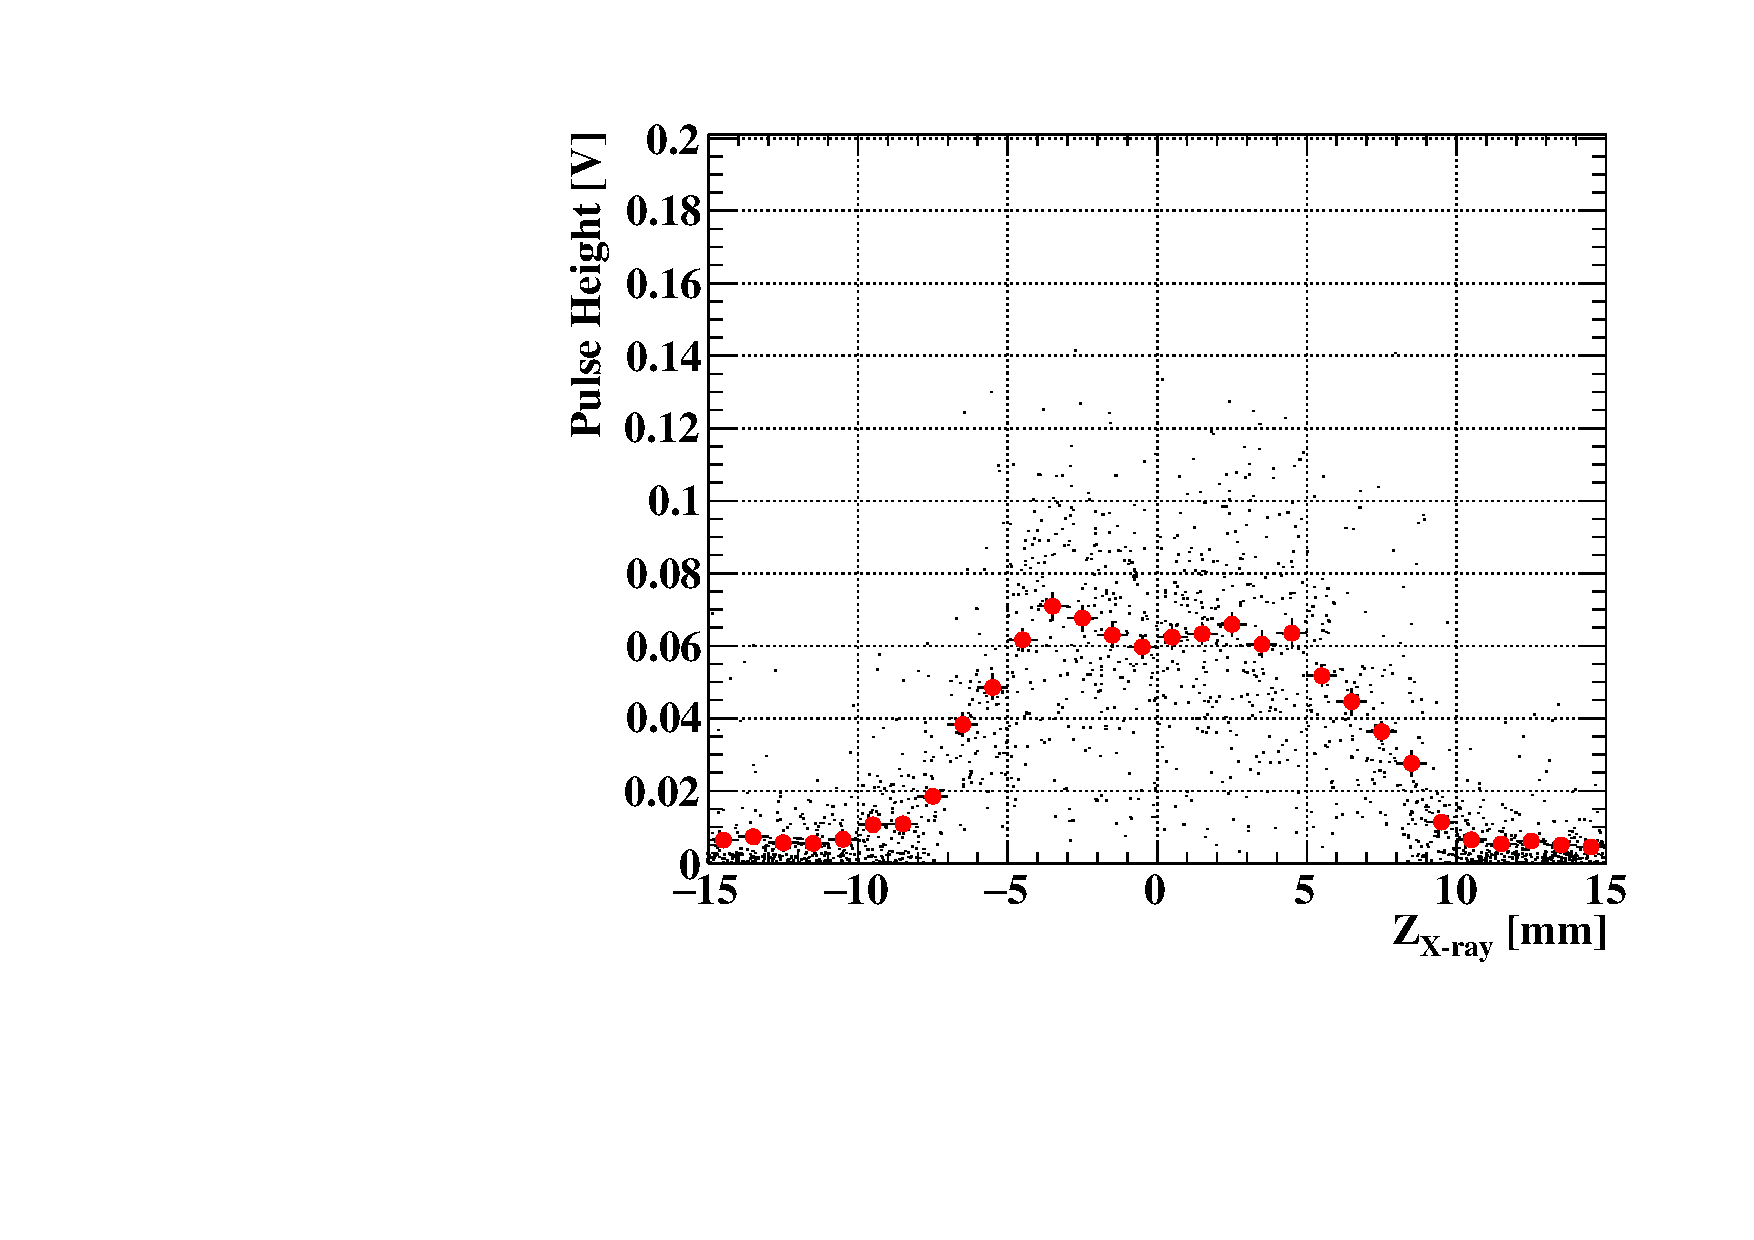
\includegraphics[width=4cm]{plots/2018/HeightvsZ}
  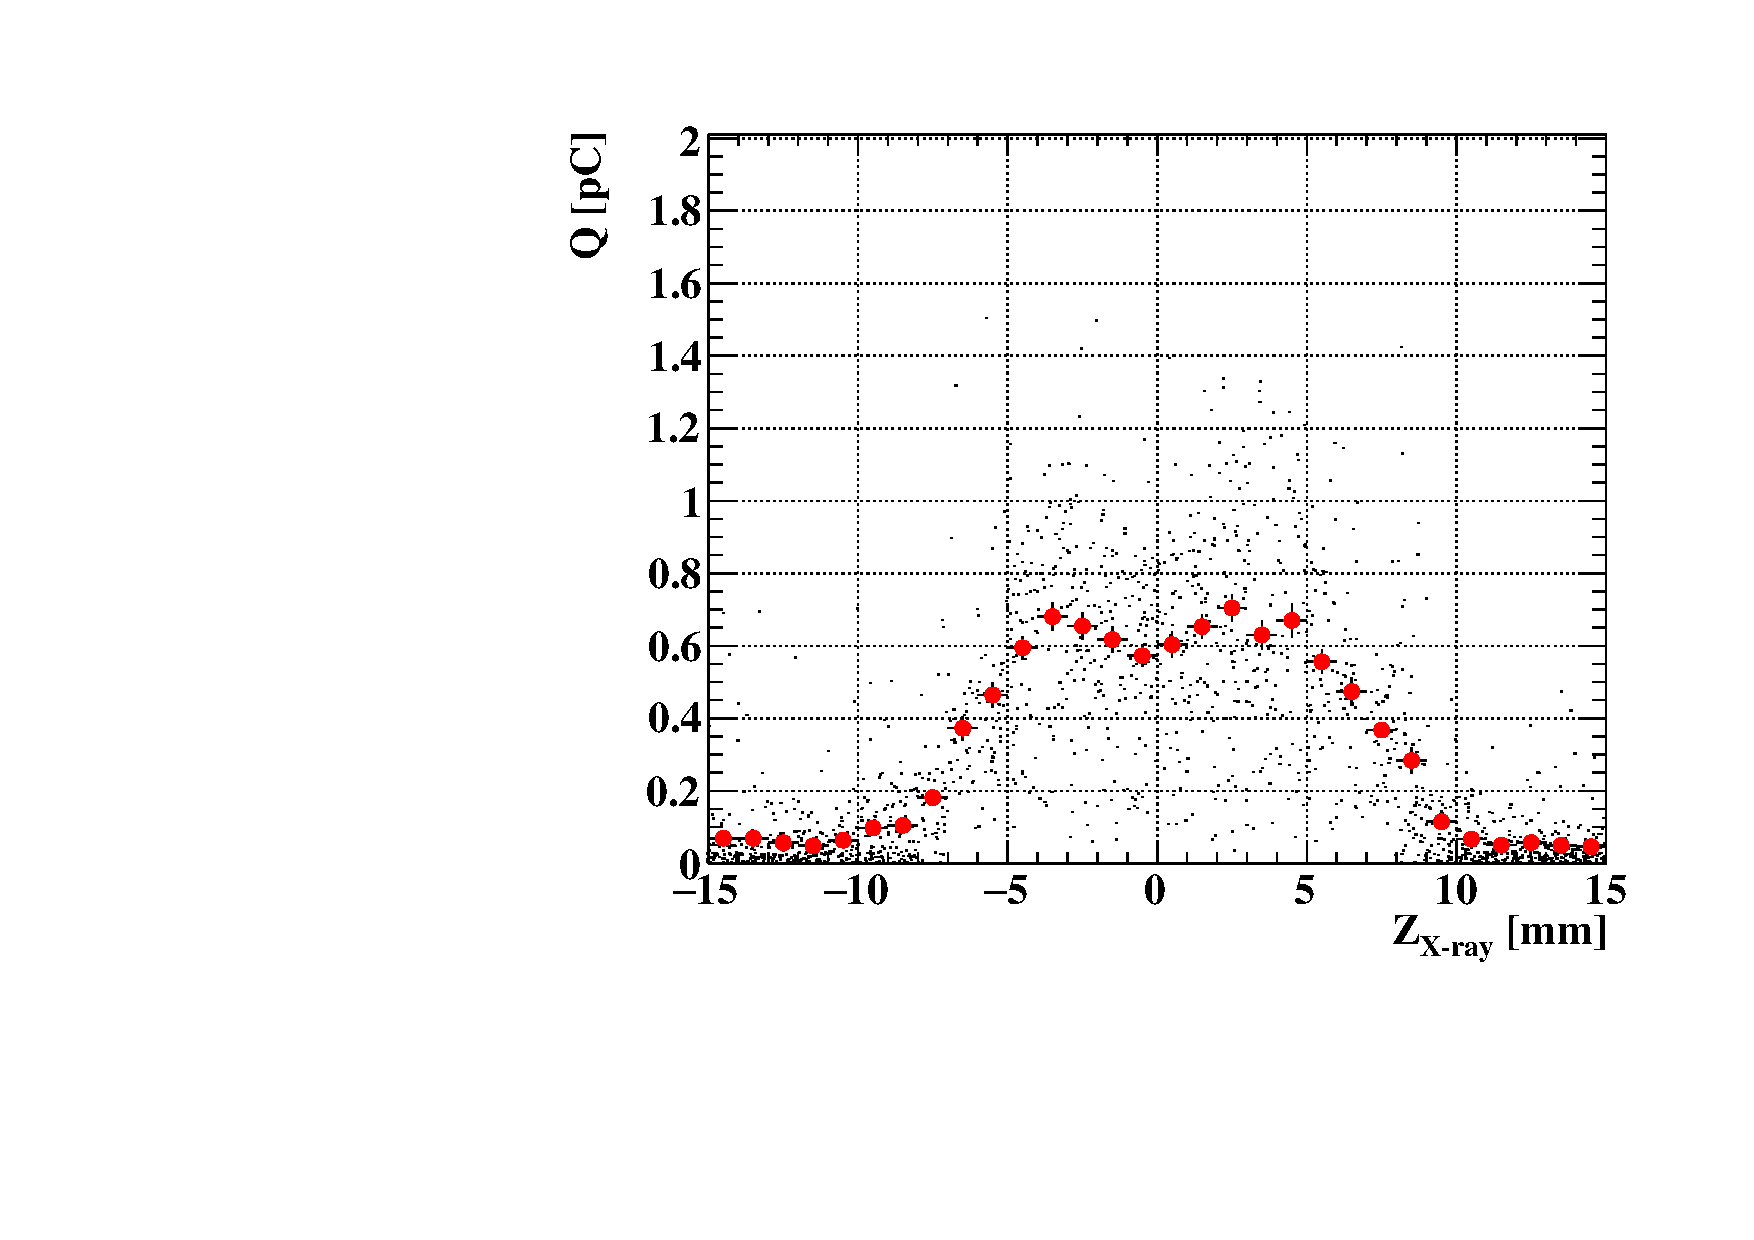
\includegraphics[width=4cm]{plots/2018/ChargevsZ}
  \caption{The waveform amplitude (left) and integrated charge (right) recorded in a single 
    photodetector as a function of the X-ray Z coordinate.
    }
  \label{fig:xrayevents}
\end{figure}  


\subsection{Z and \phis Position Measurement}\label{sec:mppcposition}
The X-ray event rate as a function of X-ray position ($z/\phi$) is
fitted with the following peicewise continuous function,\\
\begin{math}\label{eqn:mppcfitfcn}
f(z) = 
\begin{cases}
   b+s\cdot 
Exp\left[-\frac{(z - \, (\mu_m - w/2)\,)^2}{\sigma_m^2}\right] & z <
\mu_m-w/2  \vspace{3mm} \\
   b+s\cdot 
Exp\left[-\frac{(z - \, (\mu_m + w/2)\, )^2}{\sigma_m^2}\right] & z >
\mu_m+w/2    \vspace{3mm} \\
   b+s                                         & \mu_m - w/2 < z < \\
                                               & \mu_m + w/2    \\
\end{cases}
\end{math}

\noindent where, $w$ and $\mu_m$ are the width and center position of
the photodetector, $\sigma_m$ gaussian width of the edges, and $s,\,b$
are the signal and background event rates. A sample of well fitted
photodectector locations is used for  subsequent analysis.

\begin{figure}[h]
  \centering
  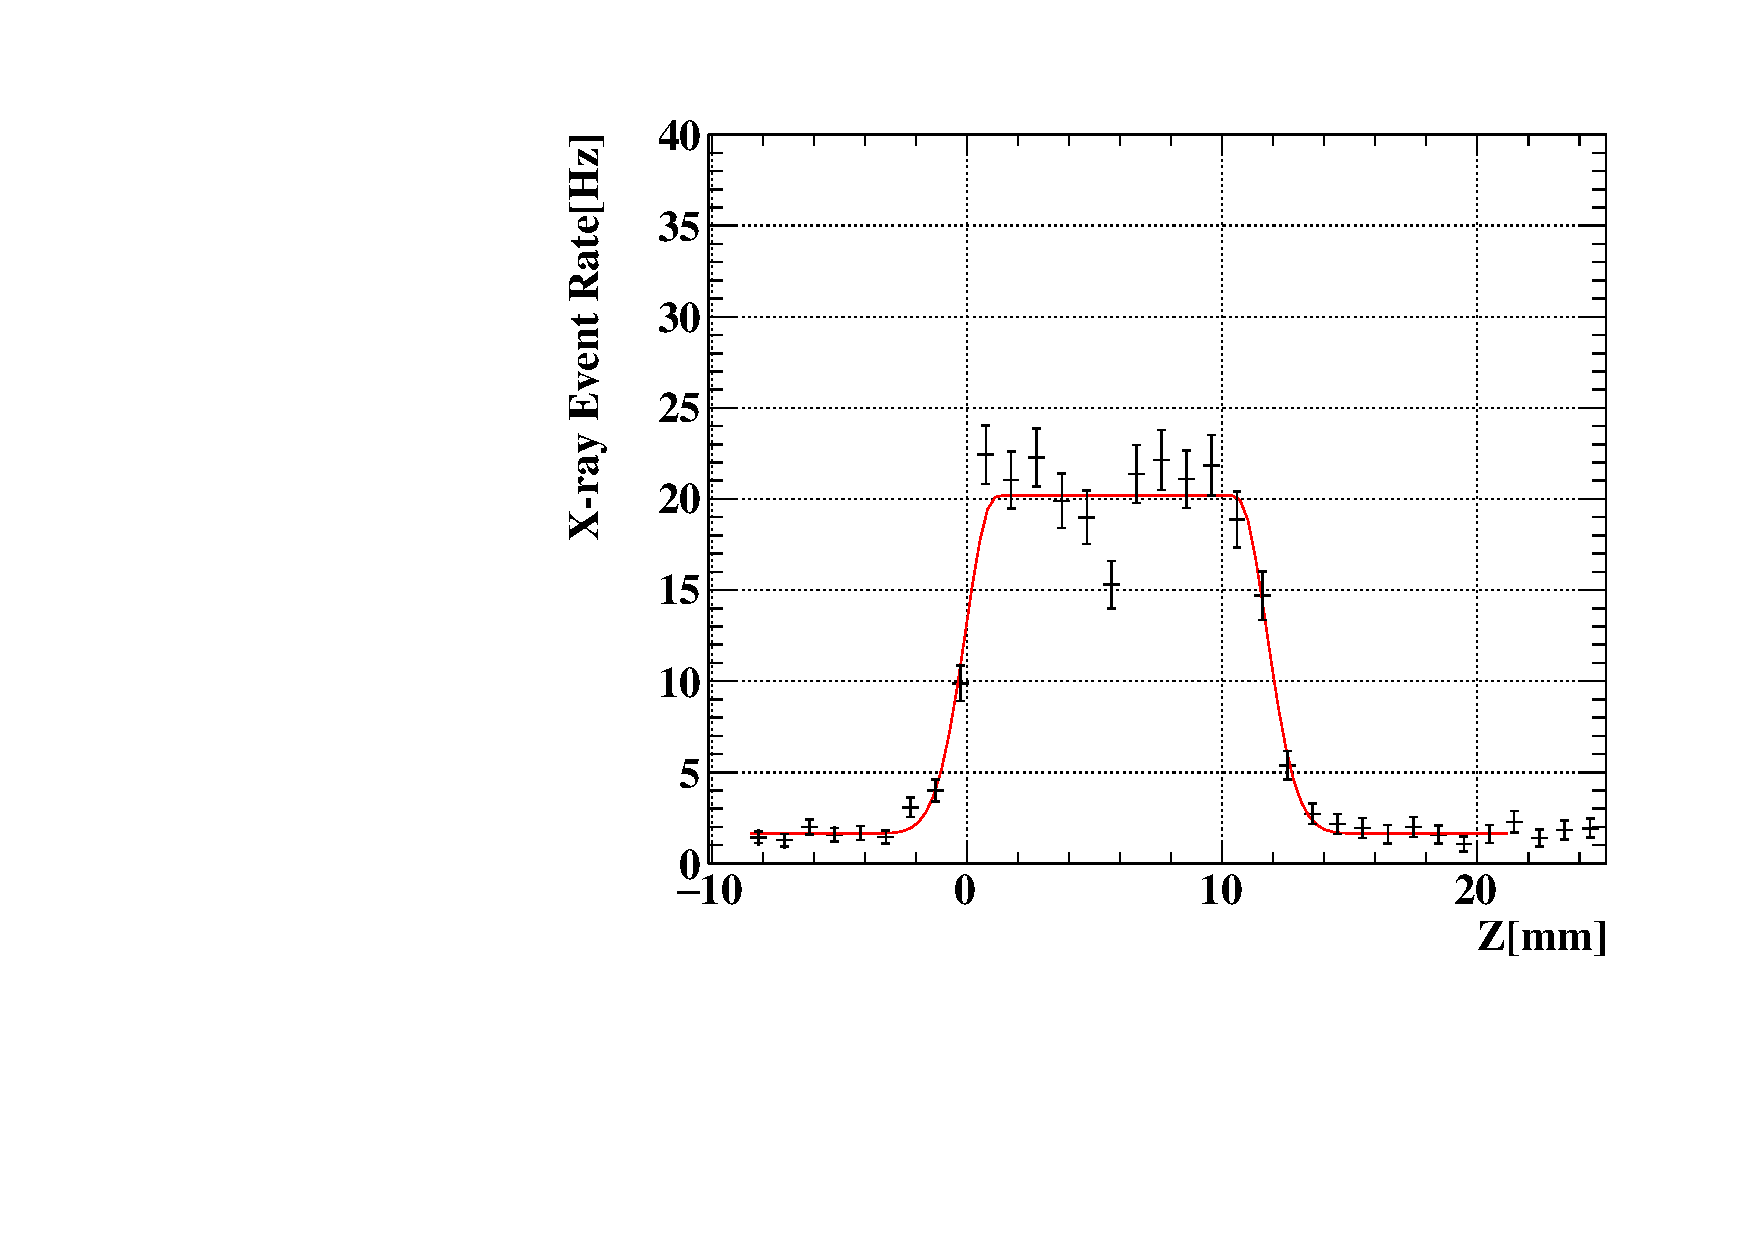
\includegraphics[width=4cm]{plots/2018/Sel5}
  \caption{X-ray event rate in a single photodetector after event selection,
    with the fit.
    }
  \label{fig:mppcfit}
\end{figure}  



The X-ray scans together with the fitted radial coordinate (described
in the next section) provide a 3D
location of each scanned photodetector  with high precision
($\sigma_{|\vec{x}|}<0.5$~mm).  These measurements are compared to a set of
nominal positions in the designed detector in order to reveal changes due to
manufacturing and installation.  Secondly, the two X-ray  measurements are
fitted to find global offsets in the absolute positions which could be
introduced due to the movement of the calorimeter or thermal cycling of LXe
scintillator conducted between the two scans.

The nominal positions of the photodetectors ($Z_{MPPC}$,
$\phi_{MPPC}$) are in a regular grid along a cylindrical surface with
constant radius, and its central axis aligned with the Z axis of the
MEG coordinate system.  From direct measurements in FARO and X-ray
surveys (described in the next section), we have shown  that the
radial coordinate of the photodetectors is not perfectly uniform.  We
find that the calorimeter can be divided into four separate regions
formed by the cfrp plates. Within each plate there is rotation of the
photodetectors about the radial axis which causes $\phi$ dependent
variation in the Z coordinate, and corresponding and equal Z dependent
variation in the $\phi$ coordinate of the MPPC measured by the X-ray
scan (figures \ref{fig:rotation1}, \ref{fig:rotation2}). The deviation of the measured from
the nominal in Z and $\phi$ coordinates is fitted independently on
mutiple subsets of photodetectors within each cfrp plate. The results
(table \ref{tab:rotation}) show the mean slope due to the rotation
varies between 2-5~mrad  or 1-4~mm displacement of the photodetector
over the entire calorimeter.
A consistently higher slope of  $d\phi/dZ$ compared to $dZ/d\phi$
indicates a 1~mrad deviation in the construction of the cfrp plate
from a perfectly 
rectilinear assembly board in the z-$\phi$ plane.  The figures and the
table show calculations using 2017 data, the results from the smaller
2018 data are found to be identical but not used. 

\begin{table}
\begin{tabular}{ccc}
   & $dZ/d\phi_{MPPC}$ & $d\phi/dZ_{MPPC}$ \\
\hline 
cfrp 1 & -0.0025 & 0.0033 \\
cfrp 2 & -0.0032 & 0.0040 \\
cfrp 3 & -0.0033 & 0.0045 \\
cfrp 4 & -0.0050 & 0.0058 \\
\end{tabular}
\caption{Average slopes (mm/mm) of deviation between X-ray and nominal MPPC positions
$dZ, d\phi$ with respect to the other coordinate, shown for each 
cfrp plate.}
\label{tab:rotation}
\end{table}

\begin{figure}
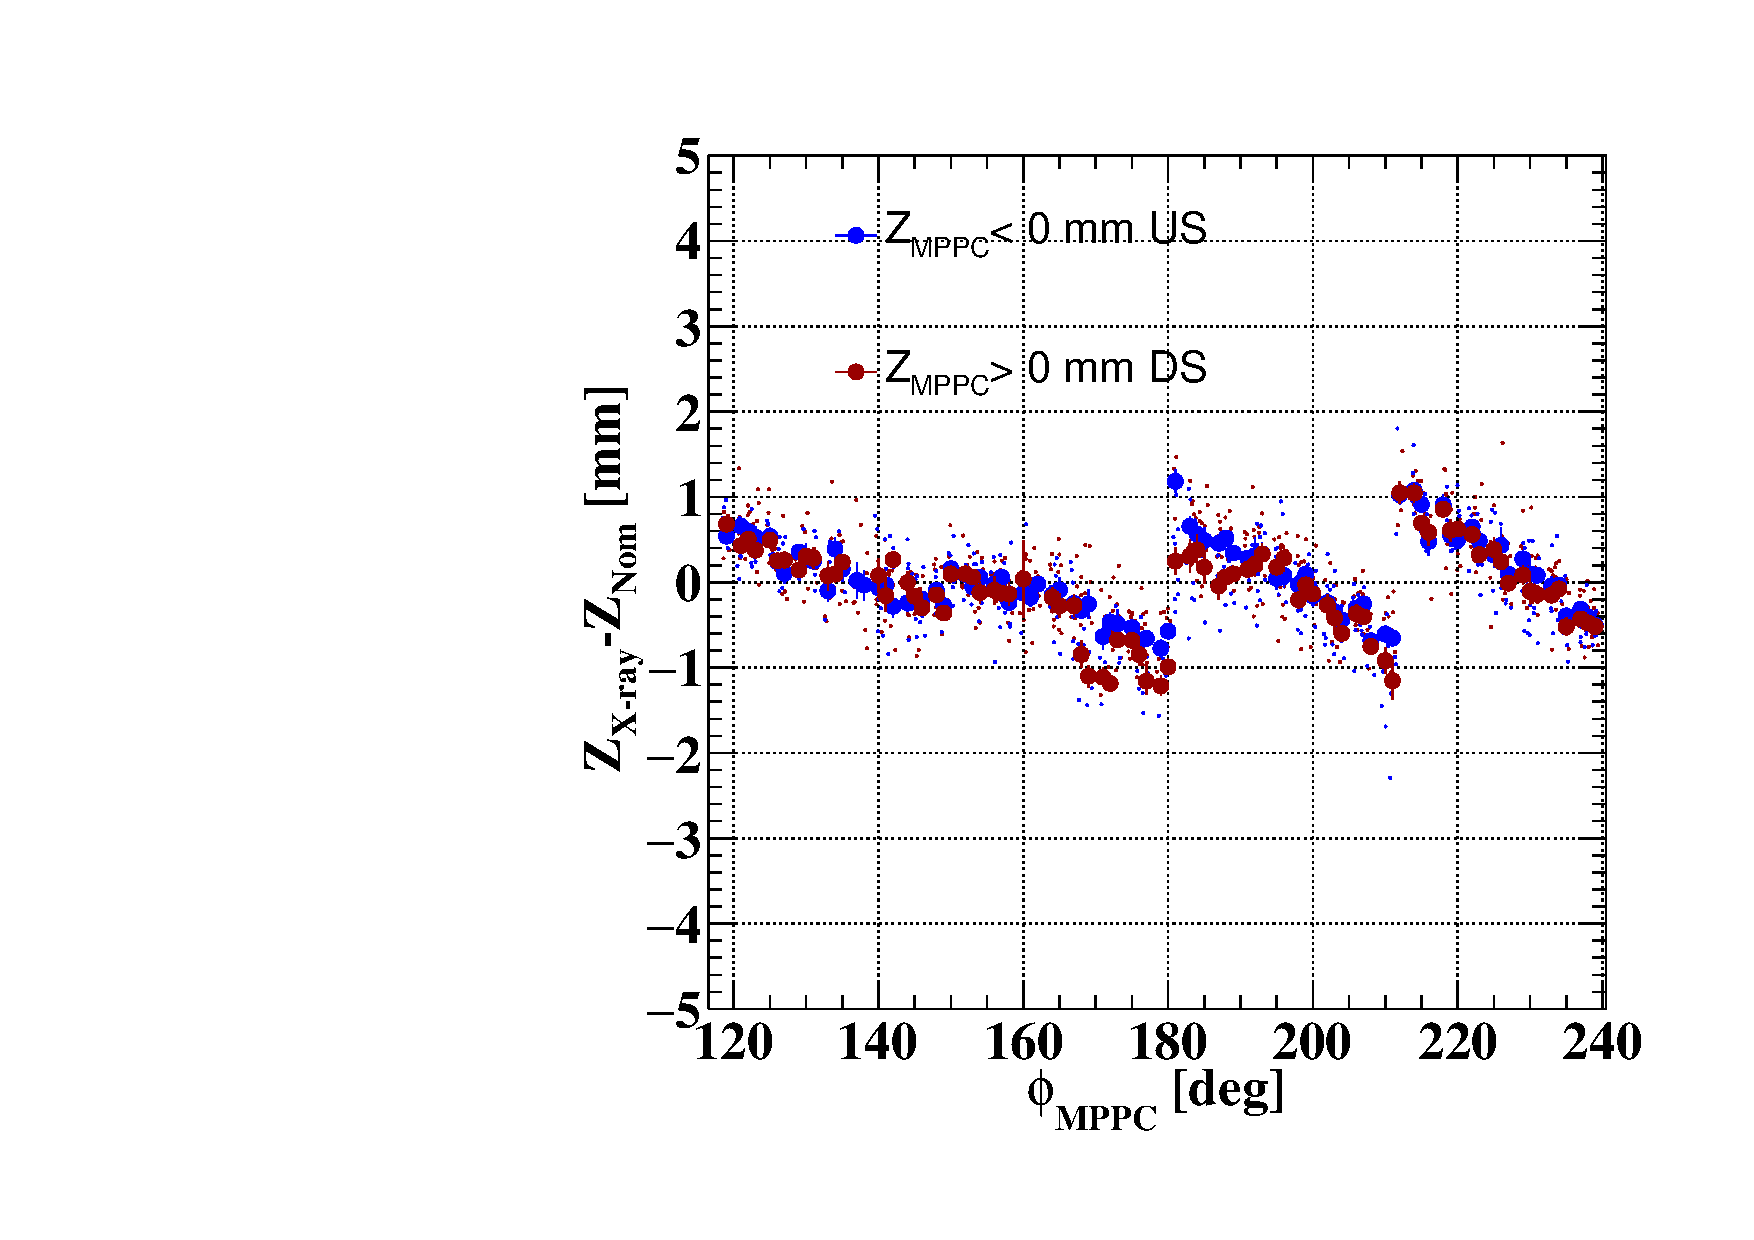
\includegraphics[width=4cm]{plots/dz_boardrotation.pdf}
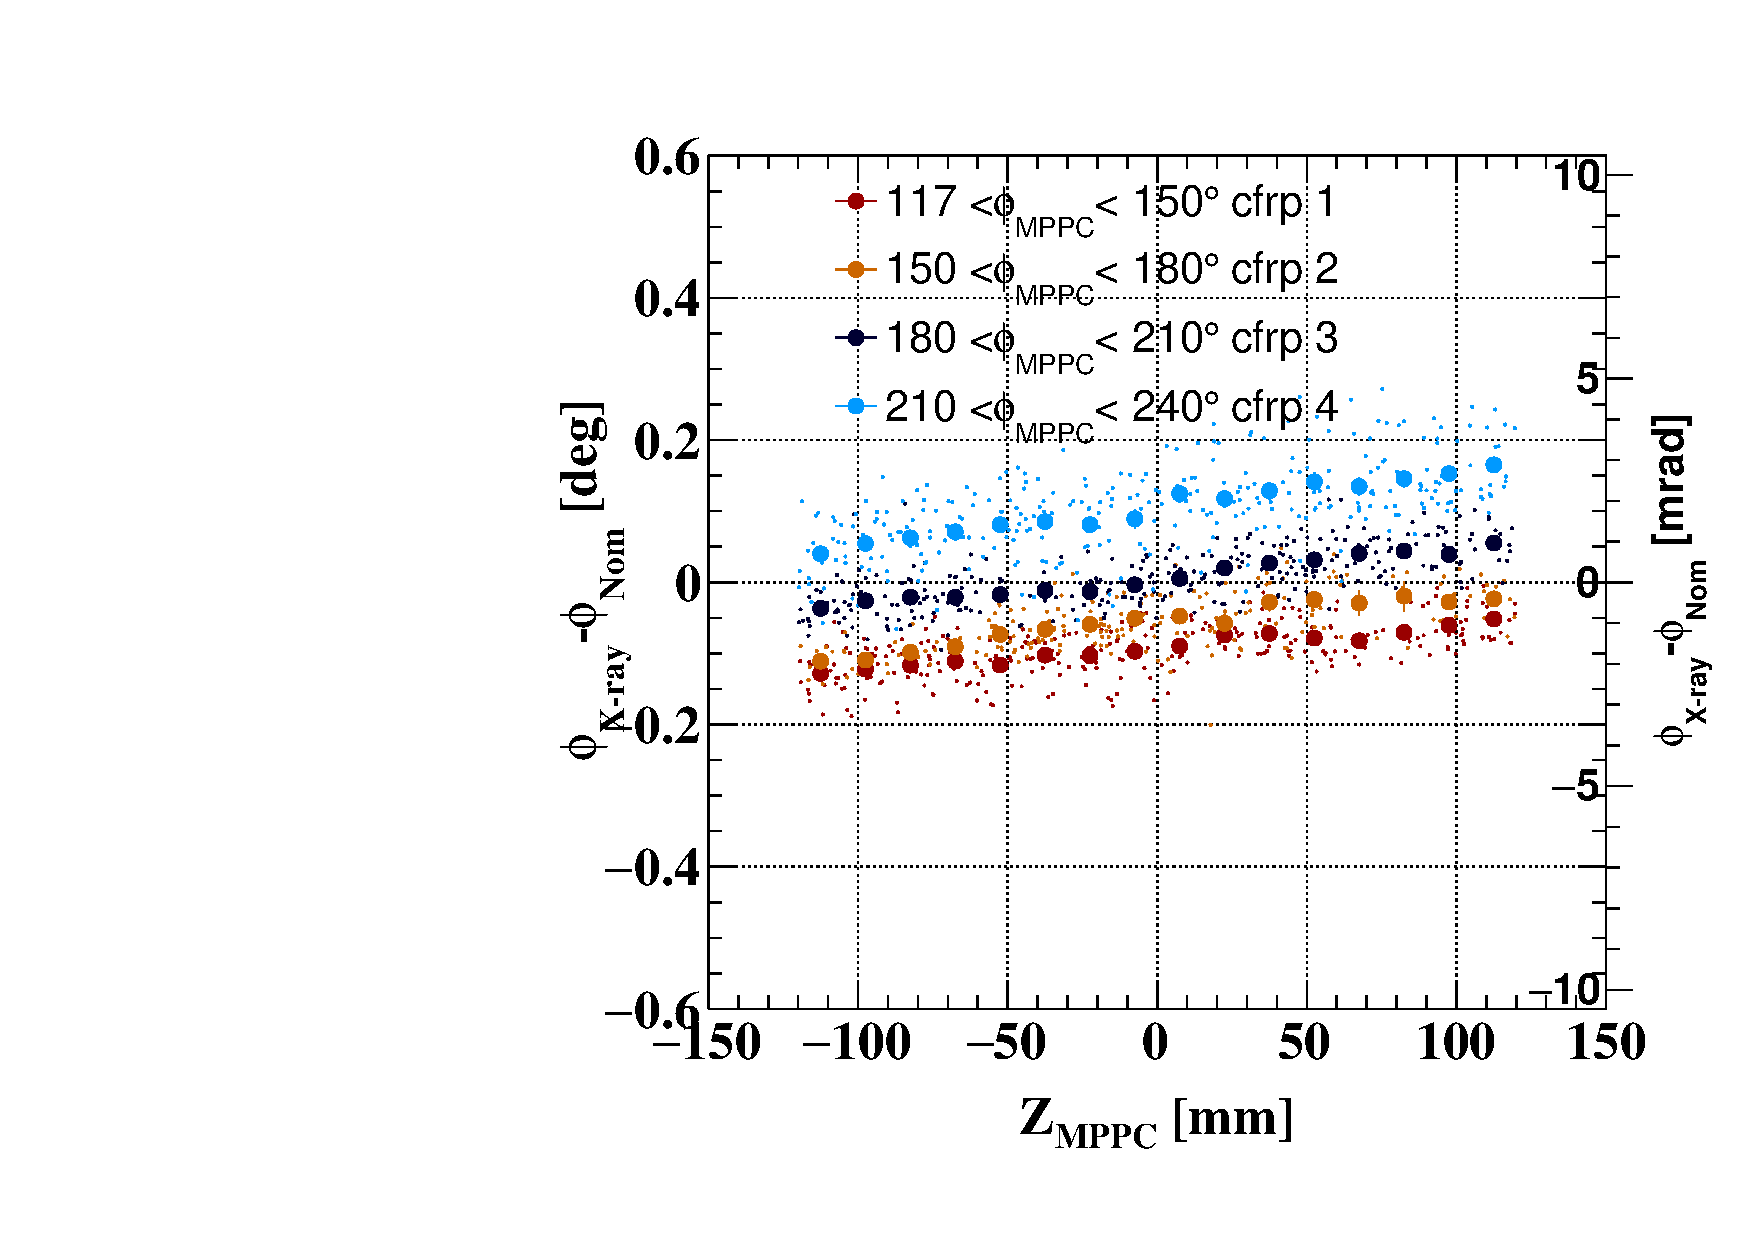
\includegraphics[width=4cm]{plots/dphi_boardrotation.pdf}\\
\caption{[add cfrp boundary]
Difference between the X-ray measured and nominal MPPC positions
overlayed with the profile histogram (scatter plots).
US and DS PCB half-strips and cfrp plates are shown separately.
Both Z and $\phi$ measurements have global offsets with respect to the 
nominal which are corrected in the plots.
}
\label{fig:rotation1}
\end{figure}

\begin{figure}
\begin{center}
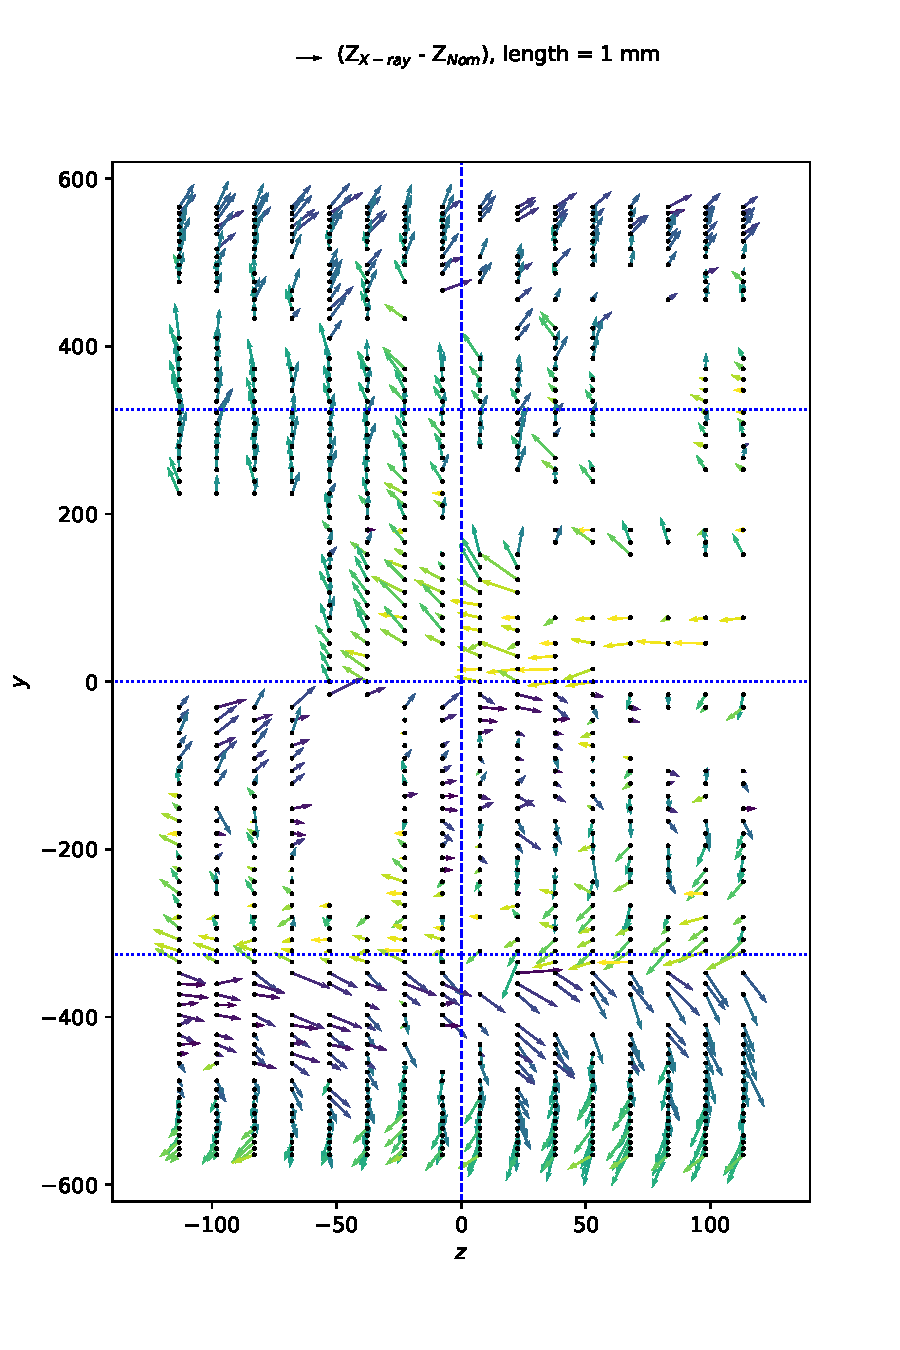
\includegraphics[width=8cm]{plots/dzdy2017_rx.pdf}
\caption{Arrow plot showing rotation of the MPPCs with respect to nominal
positions in the YZ plane; dotted horizontal lines show cfrp plate boundaries,
dashed vertical line at the center separates the PCB half-strips.
Both Z and $\phi$ measurements have global offsets with respect to the 
nominal which are corrected in the plots.
}
\label{fig:rotation2}
\end{center}
\end{figure}


The stability of the reconstructed position 
is verified by testing its dependence on 
the fitting procedure.
The pattern of X-ray event rates in each photodetector is fitted
with a different fitting function with higher-order Gaussian,

\begin{equation} \label{eqn:supergauss}
    f(z)=b+s\cdot
Exp\left[-\left(\frac{z-\mu_{m}}{\sigma_{w}}\right)^{8}\right],
\end{equation}

where $b,s$ are the signal and background event rates. The 
flat-top of the function is centered at $\mu_m$,
and $\sigma_w$ determines the size  of
flat-top as well as the gaussian width of fall-off
on both sides. 
The results show new reconstructed positions consistent with the initial
calculation with mean 0.07~mm (0.2 mrad) and standard deviation
0.3~mm (0.45 mrad)(\ref{app:fitfunccomp}).

\subsection{Spacing in Z and $\phi$}
The photodetectors are manufactured and assembled in lattice formation
to high precision, which can be used for validation of the X-ray
scanning technique and calculate its resolution.  A change in the
spacing can also reveal the effect of thermal cooling as well as
installation errors.  The spacing between individual MPPC pairs as
well as mean spacing between adjacent MPPC is calculated per PCB strip
(row-wise) along Z and per cfrp plate (column-wise) along \phis. 

Table \ref{tab:oddeven} shows spacing between individual MPPC pairs separated
into two groups which include alternate pairs along columns for Z measurement,
and rows for $\phi$ measurement.  Nominally we expect the spacing to be equal in
the two groups; the data shows the spacing in Z coordinate differs by 0.88~mm
and 0.74~mrad in the $\phi$ coordinate.  The average spacing over the scanned
region (shown in table \ref{tab:avgspacing}), however, is consistent with
expectation after accounting for thermal cooling.  
This implies a systematic shift or miscalculated position 
of one set of every other MPPC by 0.22~mm (0.18 mrad), and the oppposite 
shift for the complementary set, such there is not net displacement over the entire
row or column. 

The source of this discrepancy is not known.
Two possible causes were investigasted that could introduce observed 
systematic shifts in reconstructed MPPC positions with the periodicty of 
$\sim$30 mm, or two MPPC widths: X-ray corrections and trigger bias.
Although inaccurate corrections to the X-ray position can introduce the magnitude of 
displacement in MPPC position observed the periodicity of the corrections
does not match that of the observed effect; Z corrections have a period of 
100~mm while $\phi$ corrections are monotonic.
Similarly, studies of the effect of trigger configuration on the reconstructed position 
were not able to replicate this effect. 

As the scale of the systematic shift is small compared to the overall
X-ray measurement uncertainty as well as the precision goals of the
MEG experiment, it is expected to have minimal effect on the photon
position resolution.  We estimate this effect on photon reconstrution
using MC simulation.  A photon interaction is simulated at
normal distance equivalent to one radiation length
($\lambda_{LXe}\approx$ 2.75 cm) over a two dimensional surface
consisting of (20 $\times$ 20) photodetector array.  The dimensions and
spacing of the photodetectors are identical to the MPPC 
in the LXe calorimeter.  The isotropic distribution of photons generated as a
result is recorded by the photodetector array. The signal in each
photodetector is proportional to the solid angle subtended to the
interaction point, and detection efficiency determined by the photon
incident angle, measured in standalone tests.  
Each event is simulated with an interaction point
chosen randomly in a 30$\times$30~mm$^2$ region equivalent to two MPPC
widths, and reconstructed twice, with nominal and systematically
shifted photodetector positions by 0.22~mm.  The photon position is
reconstructed using weighted mean of the signal recorded in the
photodetectors.
The results show no mean displacement, while the photo 
position resolution is degraded by 0.08~mm in the 
measurement plane.

The mean distance between adjacent MPPCs is calculated using only the
measurements at the end of the row or column.  The precision of the
measurement is improved as a result compared to the pair-wise spacing
by  one (two) order of magnitude in Z ($\phi$).  In the Z coordinate,
the mean distance is calculated for each PCB strip as well as for the
half-strips (US and DS) connected at the center.  Similarly in the
$\phi$ coordinate, the mean distance is calculated within individual
cfrp plates and overall.  The mean and standard deviation of the
calculated mean distance in Z and $\phi$  show a regular grid
structure with no deformation in the scanned region (table
\ref{tab:avgspacing}).

The effect of thermal cooling is seen in Z with the mean distance
15.08~mm  or 30~\micron contraction between adjacent MPPCs. The mean
distance in $\phi$ is dependent on the X-coordinate of the
semi-cylindrical LXe calorimeter whose center is nominally aligned
with the center of the X-ray scanning device.  During the X-ray survey
the calorimeter was off-center, shifted towards the X-ray device by
3.85~mm increasing the mean angular spacing seen in the data.  The
following sections detail the qualitative use of X-ray data to measure
thermal contraction and 3D MPPC location.

\begin{table}
\centering
\begin{tabular}{ccccc}
 & $Z_{n}-Z_{n-1}$ &Std. Dev.& $\phi_{n}-\phi_{n-1}$ & Std. Dev. \\
 & [mm] &[mm]& [mrad]& [mrad]\\
\hline
Odd  $n$ & 15.16 & 0.32 & 23.71 & 0.78 \\ 
Even $n$ & 14.98 & 0.35 & 23.69 & 0.57 \\ 
%Nominal  & 15.1  &      & 23.55 & \\
\end{tabular}
\caption{Mean Z and $\phi$ spacing calculated for Odd-Even and Even-Odd
combination  of adjacent MPPCs.}
\label{tab:oddeven}
\end{table}

\begin{table}
\centering
\begin{tabular}{clc}
   & Z [mm] &Std. Dev. [mm] \\
\hline
US     & 15.10 & 0.05  \\
DS     & 15.06 & 0.03  \\
All    & 15.06 & 0.02  \\
Nominal& 15.1      &
\end{tabular}

\begin{tabular}{clc}
   & $\phi$ [mrad] &Std. Dev. [mrad] \\
\hline
cfrp 1     & 23.72 & 0.08  \\
cfrp 2     & 23.70 & 0.01  \\
cfrp 3     & 23.71 & 0.04  \\
cfrp 4     & 23.73 & 0.04  \\
All        & 23.72 & 0.01  \\
Nominal    & 23.55 &     
\end{tabular}
\label{tab:avgspacing}
\caption{Mean distance between adjacent MPPC calculated over the entire row (Z) or 
column ($\phi$). Upstream (US) and downstream (DS) parts of each PCB strip, and
individual cfrp plates are calculated separately, and altogether.}
\end{table}




\subsection{Charge Asymmetry} \label{sec:chargeasym}

Here, we show our previous results are consistent with
an additional measurement of each photodetector's edge location,
determined by fitting charge asymmetries (Eqn. \ref{eqn:qasym}) between
adjacent photodetectors. 
%This allows for a determination of
%photodetector edges as defined by the midpoint between two detectors,
%in which the X-ray induces charge measurements.

Event selection includes two classes of events; where the X-ray
induced charge is present in one of the channels, or shared by the two
adjacent channels.  The charge selection described in Appendix A
is expanded such that the requirement of minimal charge
can also be satisfied by the sum of charges in the two, adjacently illuminated channels.  
In order to avoid skews to the asymmetry distribution from variation in the gain
of individual photodetectors, the charge from each photodetector is
equalized by the average measured charge in events from the near half of each photodetector.
%The mean
%charge is calculated for each photodetector in the central scanning
%region and normalized before applying selection.

The charge asymmetry for a given set of photodetectors $i,j$
is calculated per event are as  
\begin{equation} \label{eqn:qasym}
    A(Q)  = 
\frac{Q_{i}-Q_{j}}
     {Q_{i}+Q_{j}}, 
\end{equation}
where $i, j$ are chosen to be adjacent photo-detector pairs 
along the direction of the coordinate scanned. The mean value
as a function of the coordinate is fitted to the 
following sigmoid function
\begin{equation}\label{eqn:asymfit}
f_{Asym}(z)=\;
C\,\left[\,Erfc(a(z-z_{0}))-1\,\right],
\end{equation} 
where $z_0$ is the offset in Z, and $C$ and $a$ are 
the scaling parameters of the function.

The center of the asymmetry distribution, $A(Q)=0$ in fig.
\ref{fig:asymplot}, constitutes the physical edge of the
photo-detector -- defined as the midpoint between active regions of the two detectors.  
The photo-detector's position and size are independently calculated in each Z and \phis coordinate as the respective average and separation of the two asymmetry edges.  A
comparison between calculated photo-detector position using X-ray event
rates and charge asymmetry (fig. \ref{fig:asymvsfit}) shows the two
measurements to be consistent.  The photodetector size 
(fig. \ref{fig:mppcsize}) is also in agreement with the
average spacing of the photodetectors previously calculated (table
\ref{tab:avgspacing}).  Due to trigger configuration and the
particular scanning region used in the X-ray survey, photodetectors on
the boundary of trigger region are excluded from the calculation,
limiting this measurement to 15\% of the scanned photodetectors.


\begin{figure}
\centering
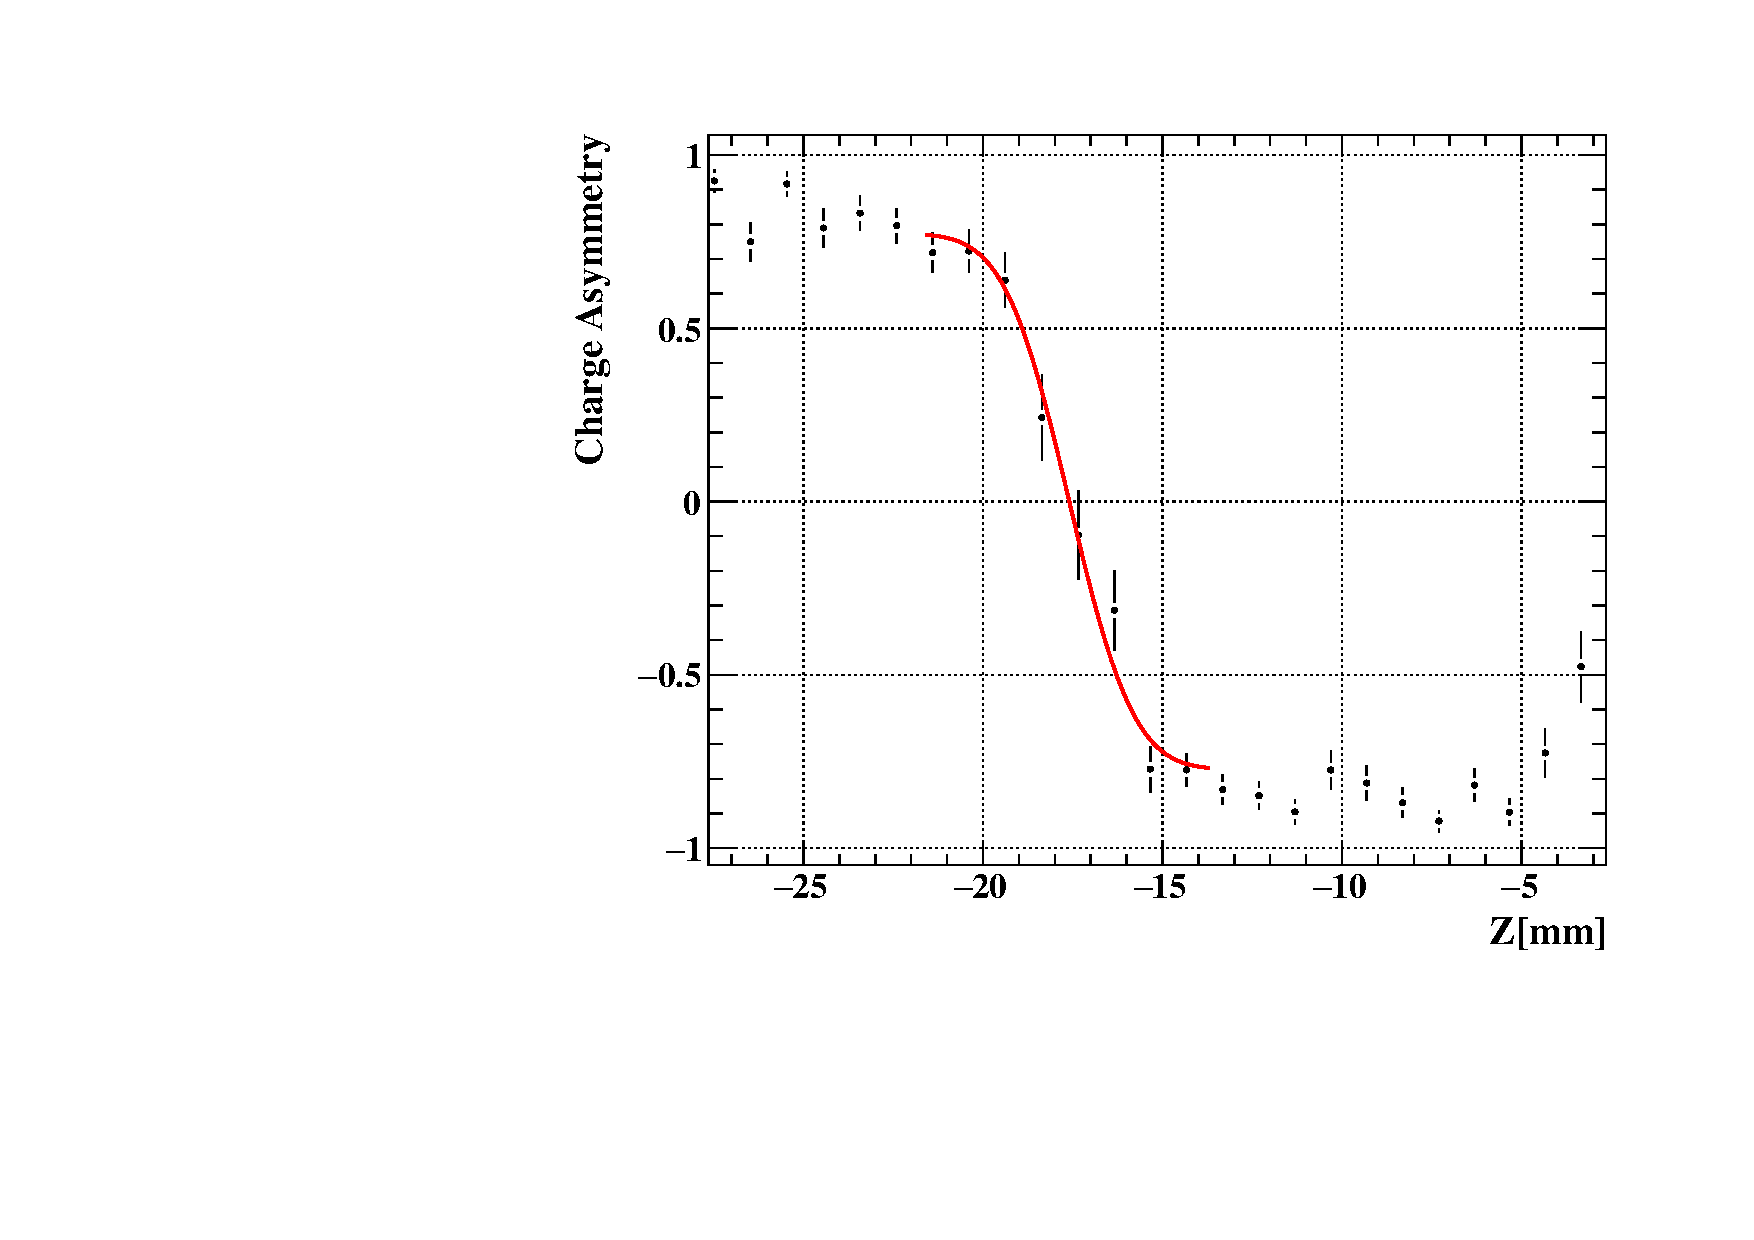
\includegraphics[width=6cm]{graphics/nnasym6465.pdf}
\caption{Mean charge asymmetry calculated as a function of z between 
two photodetectors.}
\label{fig:asymplot} 
\end{figure}

\begin{figure}
\centering
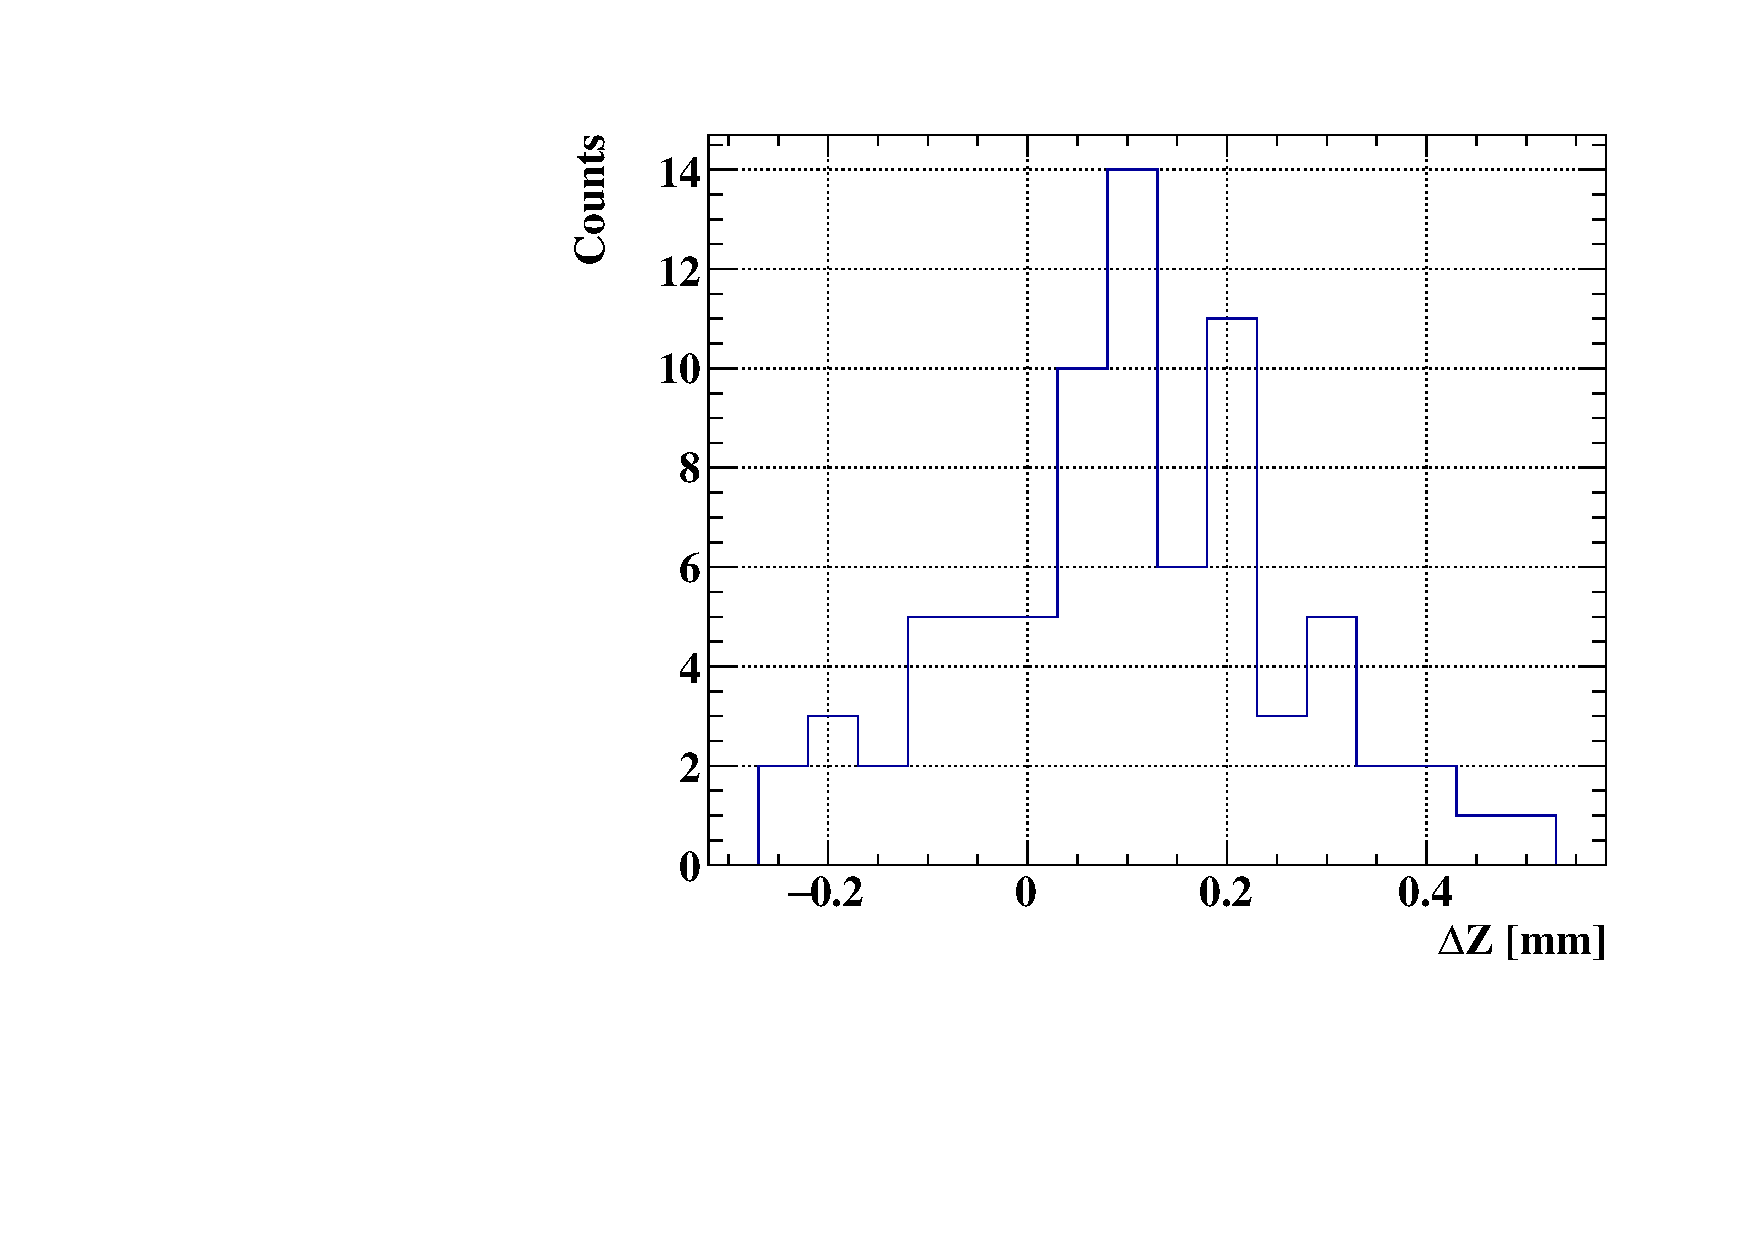
\includegraphics[width=4cm]{asymmetryplots/asymcenterdz.pdf}
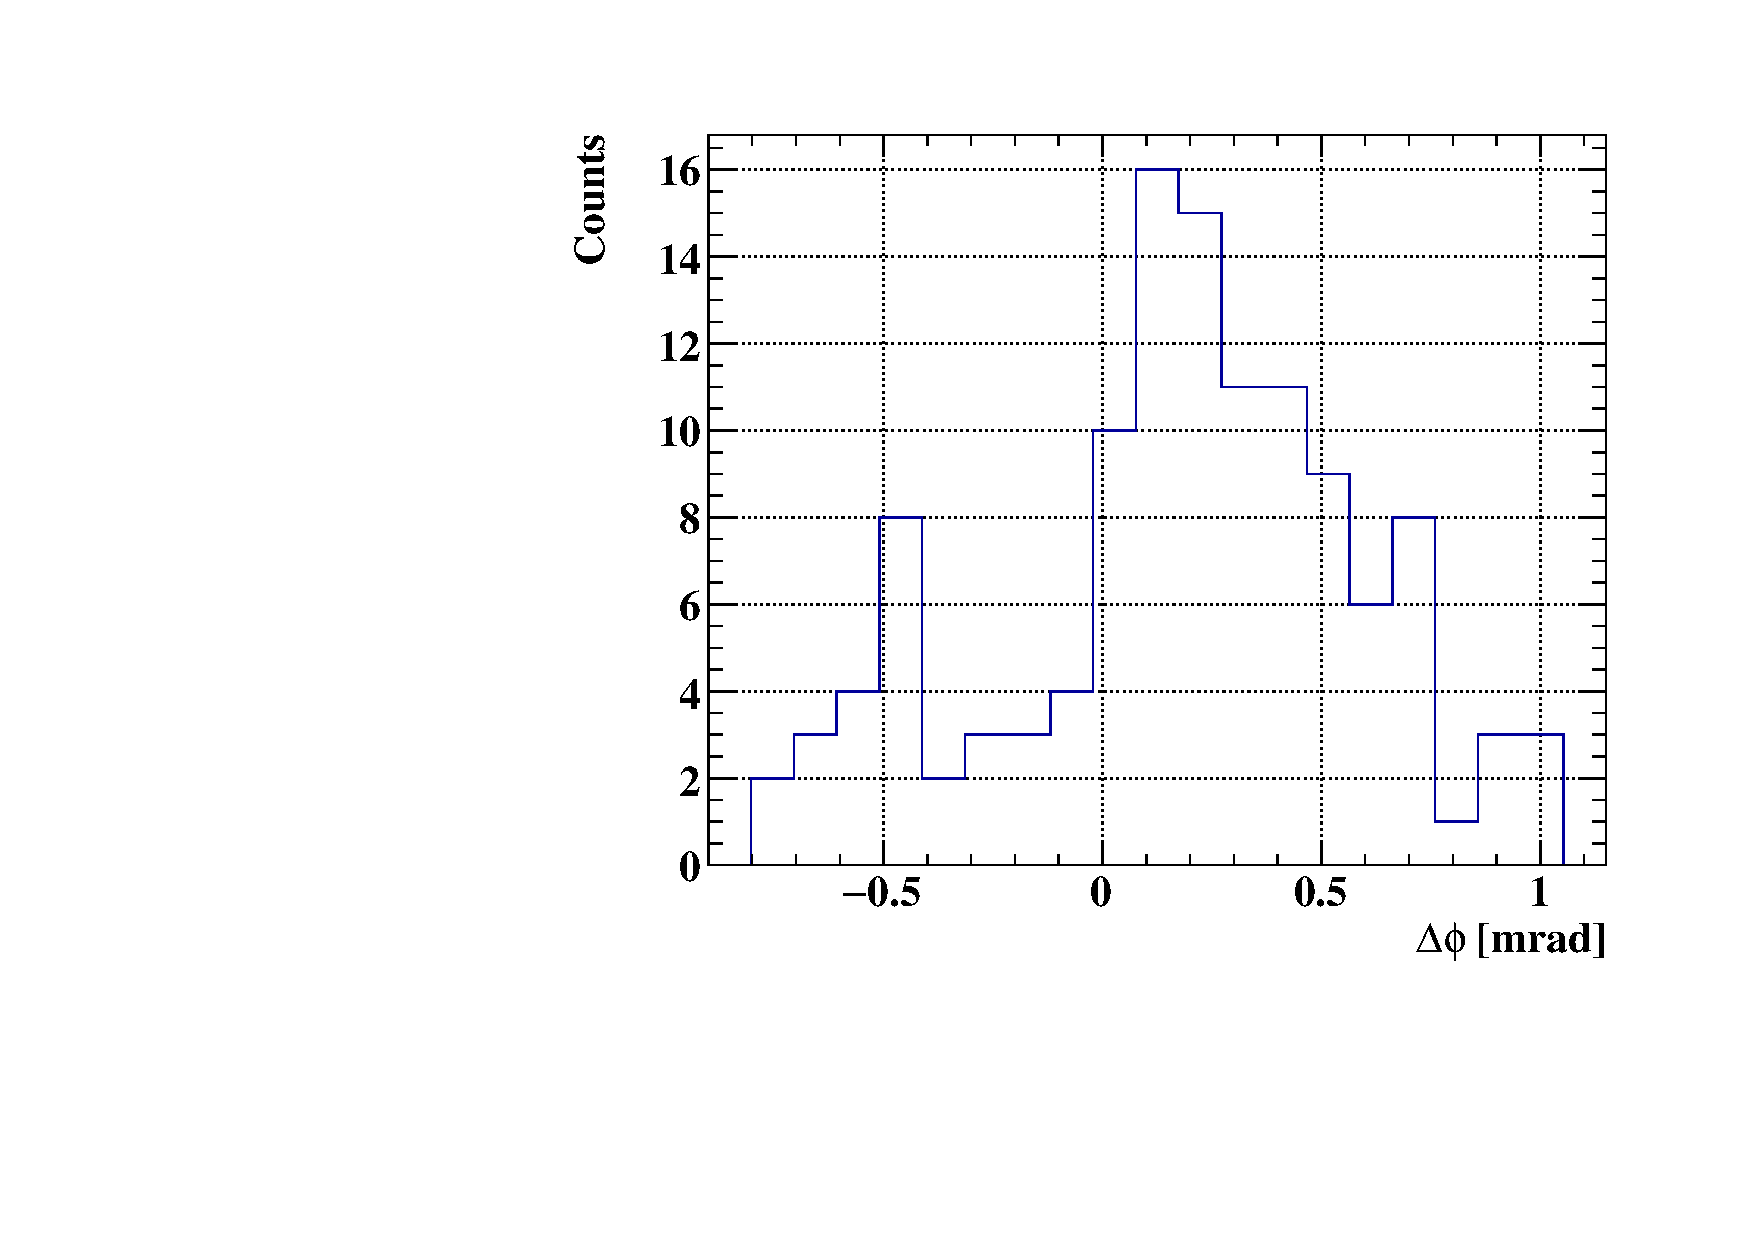
\includegraphics[width=4cm]{asymmetryplots/asymcenterdphi.pdf}
\caption{Comparison between photodetector position calculated from
charge asymmetry and X-ray event rates.}
\label{fig:asymvsfit} 
\end{figure}




\begin{figure}
\centering
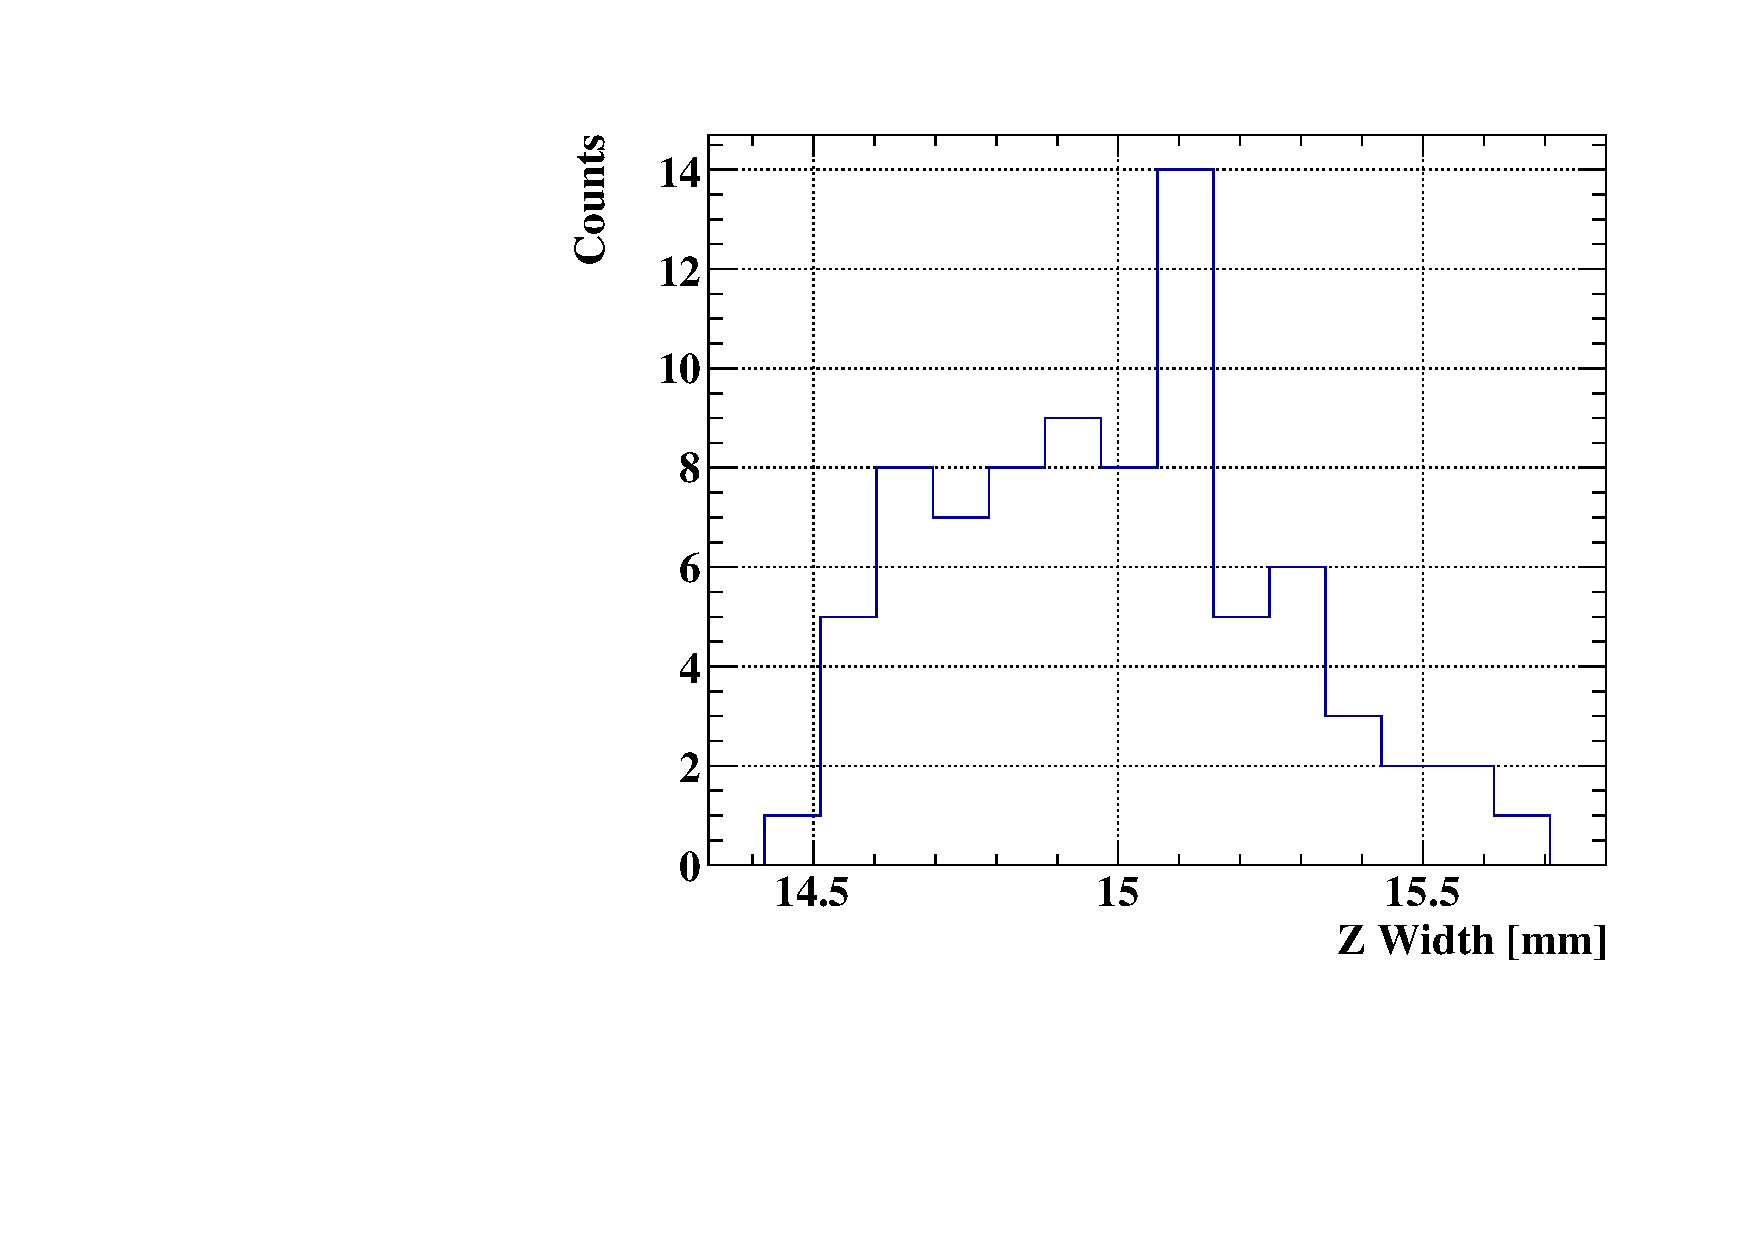
\includegraphics[width=4cm]{asymmetryplots/asymzwidth.pdf}
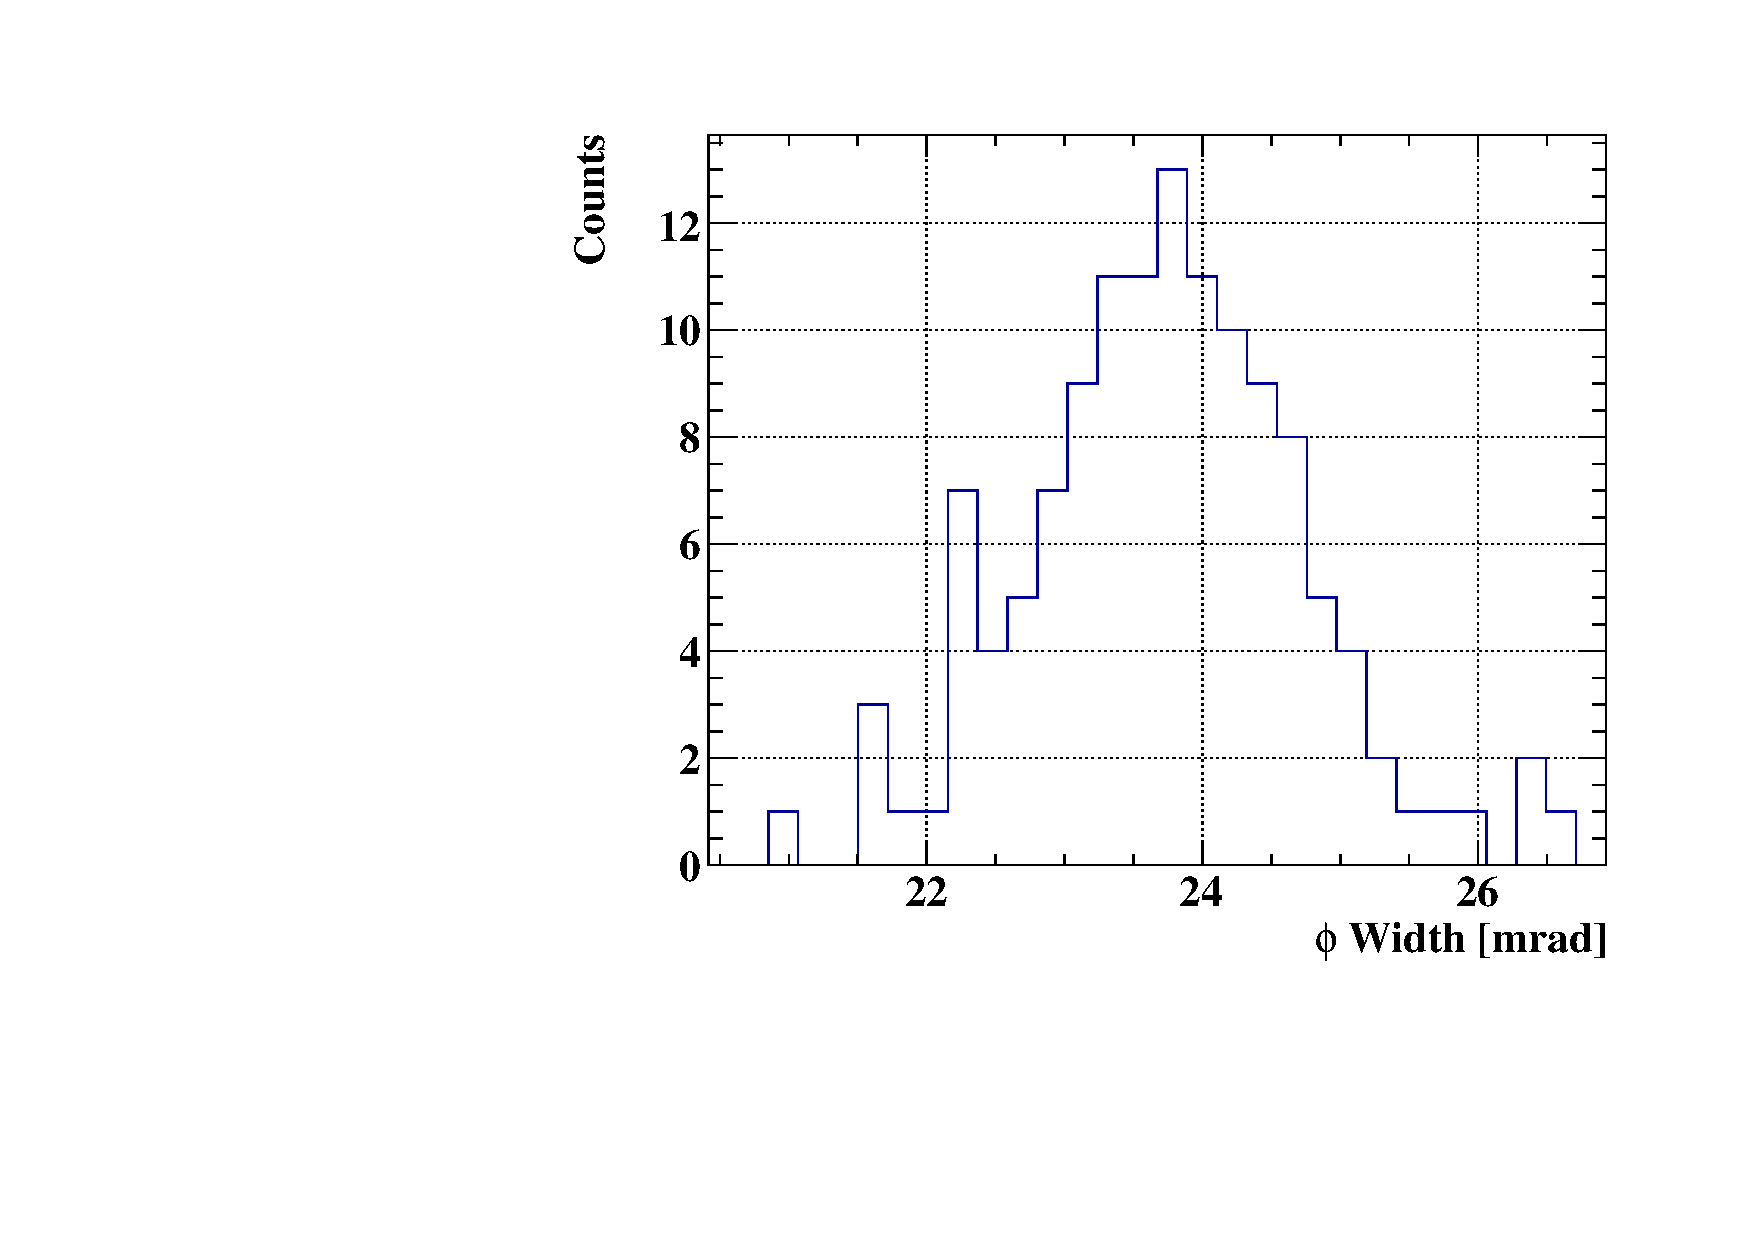
\includegraphics[width=4cm]{asymmetryplots/asymphiwidth.pdf}
\caption{Photodetector size in Z and phi measured using the edge of the
photodetector calculated with charge asymmetry.}
\label{fig:mppcsize} 
\end{figure}


\subsection {R coordinate calculation and 
coefficient of thermal expansion}
The radial coordinate not directly measured in the X-ray scan is
calculated using information from the FARO scan of the photodetectors.
The FARO scan provides highly precise 3D coordinates
($\sigma_{|\vec{x}|}$ = 200 \micron) of a subset of photodetectors
(10\%) measured at room temperature. To determine the position of
every photodetector, these measurements are interpolated by fitting
the 3D surface formed by the photodetectors. The radial coordinate and
center are calculted first with a cylindrical fit function, followed
by z,$\phi$ coordinates fitted to a regularly spaced grid in z-$\phi$
plane allowing for small rotations in the plane.  Each cfrp plate is
fitted independently since the curvature varies slightly between
individual plates and the overall curvature of the calorimeter.  


The interpolated photodetector locations from FARO
and X-ray scans are fitted with degrees of freedom to account for
global translational motion, extrinsic rotation centered in the MEG
coordinate  system, and scale factor for thermal contraction. 
The FARO coordinate is transformed using the equation
\begin{align}
\vec{x}_{FARO}^{'} = (1-s)R(\alpha,\beta,\gamma)\vec{x}_{FARO} +
\vec{x}_{offset},  
\end{align}
where $s$ is the scale of thermal contraction, $R$ is the rotation
matrix  and $\vec{x}_{offset}$ is the linear offset. 
The fit parameter values are extracted by minimizing the following function
\begin {align}
\chi^2 = 
\sum\limits_{i}^{N_{MPPC}} \frac{(Z_{i}^{Xray}-Z_{i,FARO}^{'})^2}{\sigma_{Z_{i}}^2} 
+ 
\frac{(\phi_{i}^{Xray}-\phi_{i,FARO}^{'})^2}{\sigma_{\phi_i}^2},
\end{align}
where $\sigma_{Z_i}$ and $\sigma_{\phi_i}$ include the resolution
of X-ray and FARO measurements
added in quadrature: 
$\sigma^{FARO}$ = 0.14~mm (0.25~mrad), 
$\sigma^{Xray}$ = 0.40~mm (0.56~mrad),
calculated from adjacent MPPC spacing described above.


The radial values from the FARO measurement are transformed using
fitted parameters to calculate radial coordinate of each
photodetector.  The uncertainty is calculated using linear error
propagation and corresponds to change in the main result due to one
standard deviation variation in the parameters taking correlations
into account.  The results in table \ref{tab:radius} shown mean radius
648.7 and 644.9~mm,and mean error 0.16 and 0.27~mm respectively in the
two scans(figure~\ref{fig:radiuscalculation}).  The radial coordinate
change of 3.8~mm between the two scans is consistent with the shift of
equal magnitude (3.85$\pm$0.1~mm) in the X-coordinate of the LXe
calorimeter in the same period.  A $\phi$ dependent change in the
radial coordinate is seen in 2018 data compared to the previous year's
data due to the calorimeter center offset with respect to the X-ray
device in 2018.



The thermal expansion coefficient is calculated as
\begin{align}
 s= \alpha_t \, \Delta T,
\end{align}
where s is the scale of thermal contraction, $\alpha_t$ is coefficient
of thermal expansion and $\Delta T$ is the change in temperature. 
Using $\Delta T$ ( = 123$\pm$10 K) 
between FARO survey performed at room temperature
(293 K) and X-ray survey performed at LXe temperature (170 K)
the thermal coefficient is calculated in the
two X-ray surveys (table \ref{tab:thermalcoefficient}).
\begin{table}[h]
\centering
\begin{tabular}{ccc}
Scan Period & $s$ & $\alpha_t \,\, [\mathrm{ppm K}^{-1}]$\\
\hline
2017 & 0.0014(1) & 11.0$\pm$1.4 \\
2018 & 0.0018(2) & 14.5$\pm$2.2 
\end{tabular}
\caption{Fitted scaling parameter ($s$) and the calculated thermal 
expansion coefficient.}
\label{tab:thermalcoefficient}
\end{table}
The theoretical value of $\alpha_t$ for the
detectaor material is 16$\pm$1 ppmK$^{-1}$.



\subsection{Change in MPPC postion 2017 vs 2018}
The photodetector positions measured from the two X-ray surveys are
compared using the same fitting procedure to verify the stability 
of the photodetector ensemble.
The motion between the two
must be understood relative to the motion of the LXe calorimeter
position which has also moved between the two surveys.  Multiple
positions on the external surface of the calorimeter were optically
surveyed before each X-ray survey to record its location.  
Overall the motion of the calorimeter is replicated well 
by the photodetectors (table \ref{tab:xray2017vs2018}),
characterized by small angular rotations, and 
large displacement along X-axis seen in both data. 

\begin{table}[h] 
\centering
\begin{tabular}{rrrrr} 
Fit Paramter &  X-ray & Unc & 
Optical & Unc \\ 
\hline 
dx [mm]   &   3.783 & 0.034 &      3.857 &  0.505     \\ 
dy [mm]   &  -0.923 & 0.114 &     -1.179 &  1.509     \\ 
dz [mm]   &  -0.885 & 0.019 &      0.144 &  1.362     \\ 
rx [mrad] & -29.378 & 3.807 &   1369.871 &  4.456     \\ 
ry [mrad] &  -0.008 & 0.051 &     -0.251 &  1.093     \\ 
rz [mrad] &  30.095 & 3.807 &  -1370.741 &  4.456    

%%lxe
%%  1  rx          -4.98974e-05   1.12590e-04   1.81586e-08  -5.11285e-04
%%   2  ry          -2.46074e-04   1.69744e-04   8.54602e-09   1.55717e-02
%%   3  rz          -8.69646e-04   1.75347e-04   8.56504e-09   2.63737e-03
%%   4  dx           3.85602e+00   7.18101e-02   3.55683e-08   1.44061e-03
%%   5  dy          -1.18210e+00   2.30683e-01   3.55680e-08   7.98124e-04
%%   6  dz           1.45227e-01   2.24210e-01   3.55680e-08   3.00940e-03
%%
%%xray
%%   1  rx          -9.03902e-05   1.03847e-04   2.07576e-07  -4.03030e-03
%%   2  ry           1.73869e-04   3.56954e-04   1.50140e-07   8.05430e-03
%%   3  rz          -3.49186e-04   3.02230e-04   1.19763e-07  -2.19844e-02
%%   4  dx           3.83337e+00   6.64374e-02   4.16831e-07   2.82117e-03
%%   5  dy          -6.77152e-01   2.39740e-01   3.01004e-07   9.43571e-03
%%   6  dz          -9.02411e-01   1.90330e-01   2.49133e-07   5.52444e-03
\end{tabular}
\caption{Fit parameters denoting change in position of the calorimeter
(from optical survey) and the photodetector position (X-ray survey),
between the two data-taking periods, 2017 and 2018.}
\label{tab:xray2017vs2018} \end{table}



\begin{table}
\centering
\begin{tabular}{ccc}
 & $R^{2017}$ & $R^{2018}$   \\
\hline
cfrp 1 &  649.3  & 645.8  \\
cfrp 2 &  648.8  & 644.7  \\
cfrp 3 &  648.5  & 644.9  \\
cfrp 4 &  647.8  & 645.7  \\
Average&  648.6  & 645.2  \\
\end{tabular}
\caption{Mean radius and error in mm in each cfrp plate for the two X-ray scans.}
\label{tab:radius}
\end{table}

\begin{figure}
\begin{center}
%\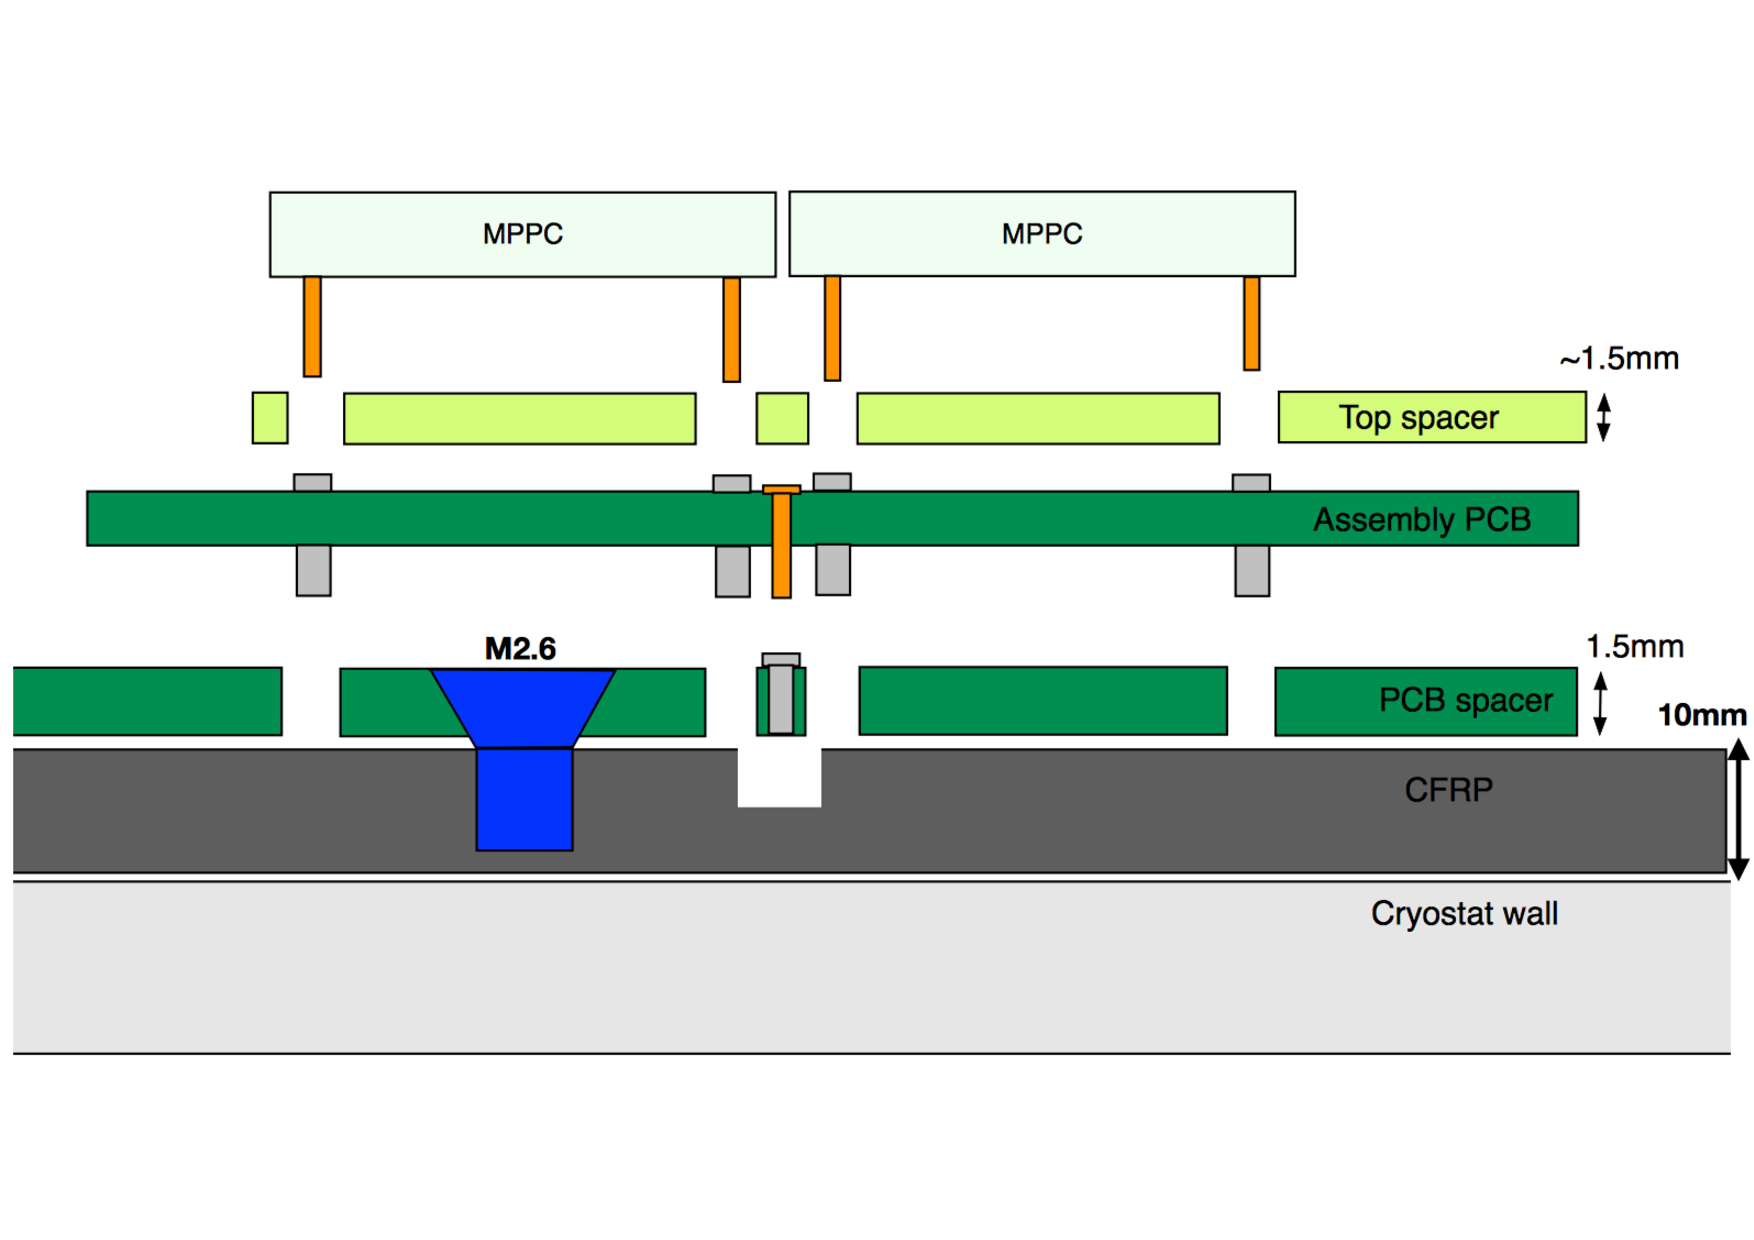
\includegraphics[width=4cm]{plots/MPPC_support.pdf}
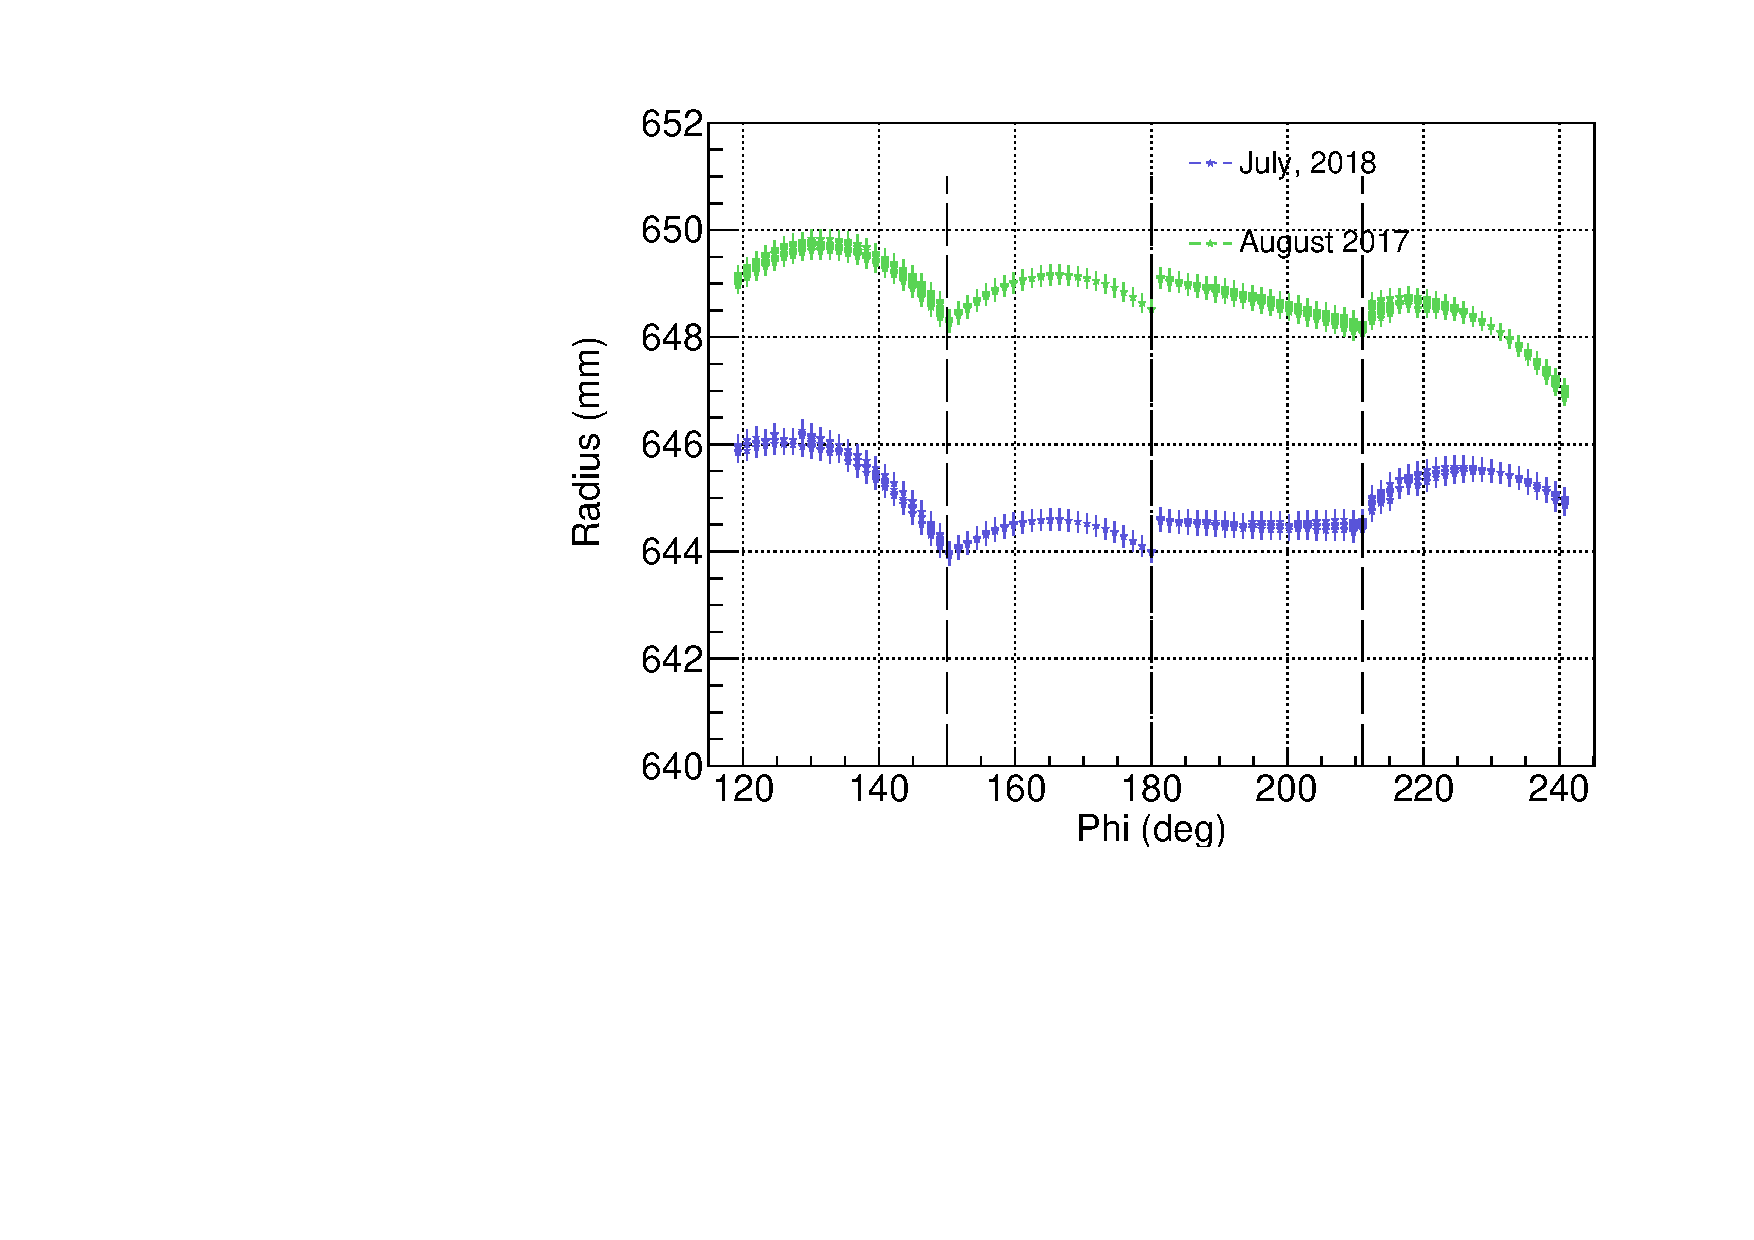
\includegraphics[width=4cm]{plots/2018/cRadius_1718}
\caption{ Radial coordinate of photodetectors with errors from 2017 and 2018
X-ray scans.  Black dashed lines indicate the edges of the CFRP plate.}
\label{fig:radiuscalculation} 
\end{center}
\end{figure}



\subsection{Uncertainties}\label{sec:uncertainties}
The uncertainty in the measured positions comes from the
precision of alignment of the X-ray device, and resolution of the
rotation angle monitoring instruments. The optical survey used
for the alignment has resolution of 0.1~mm in each coordinate
(x,y,z), which directly affects the Z coordinate of the
measurement. The error in X-ray $\phi$ coordinate due to
misalignment of the X-ray device is not easily evaluated as it
varies with $\phi$.  The maximum deviation over the scanning
$\phi$ range due to variation in (x,y) in the following
combinations is  considered as $\phi$ uncertiainty:
(0,$\pm\sigma_{xy}$),($\pm\sigma_{xy}$,0),
($\pm\sigma_{x}$,$\pm\sigma_{y}$), where $\sigma_{xy} =
\sqrt{\sigma_{x}^{2}+\sigma_{y}^2}$.

The rotation angles about all three axes are monitored using the
laser system as well as the buble-level, and provide Z and $\phi$
dependent corrections to the X-ray coordinates.  The uncertainty
on the x,y rotations come from variation in the recorded laser
intensity.  The corresponding uncertainty in the Z correction is
calculated to be 0.03~mm (6\%), varying with both X-ray
coordinates.  The z rotation is measured by the bubble-level with
0.08~mrad (13\%) uncertainty, defined as maximum deviation in the
measured values at each Z position  over mutiple runs throughout
the data-taking period.  The statistical uncertainty in the
photodetector position is introduced due to fluctuation in the
number of X-ray interactions. The interaction rates are measured
with 10\% precision leading to statistical uncertainty in the
fitted position of  0.11~mm (0.16~mrad).  A summary of all
uncertainties contributing to the measured Z and $\phi$ positions
with 2018 data is given in table~\ref{tab:uncertainties}; similar
results determined with 2017 data are shown.

A measure of overall precision of the measurement can be
estimated using spacing of adjacent MPPC pairs calculated in
table~\ref{tab:oddeven}.  We expect the spacing to be uniform and
infer the precision of the single measurement based on the
standard deviation of the pairwise spacing. Conservatively, the
calculation shows $\sigma_Z$= 0.40~mm and $\sigma_\phi$=
0.56~mrad, higher than expected from the systematic and
statistical sources considered indicating that there are
additional sources of uncertainty which are not included. The
precision, however, is within the experimental goals as well as
the aims of this X-ray survey.

An alternate means of validation of the X-ray measurement is
provided by the lead absorber strips attached to the front face
of the LXe cryostat (fig \ref{fig:lead1}), which can be located
independently by X-ray and optical surveys.  Eight thin strips
(30$\times$3 mm$^2$) are placed lengthwise along $\hat{z}$ or
$\hat{\phi}$ direction each.  Scanning with X-ray shows a deficit
of interactions in the photodetector due to X-ray absorption,
which is fitted with a gaussian shape added to the photodetector
fitting function described in sec.\ref{eqn:mppcfitfcn}.
Comparison of the X-ray and optical survey measurements of strip
positions show good agreement, with standard deviation
$\sigma_Z$= 0.41~mm and $\sigma_\phi$= 0.67~mrad, comparable to
the one observed with MPPC spacing.  The results are included in
table \ref{tab:uncertainties} and shown in figure \ref{fig:lead2}.

\begin{table}
\begin{tabular}{clcc}
 & Source & Z Unc [mm] & $\phi$ Unc [mrad] \\
  \hline
1& Alignment      & 0.1  & 0.21  \\
2& Fit           &  0.11 & 0.16  \\
3& Laser System  &  0.03 &  - \\
4& Bubble-level  &  -    & 0.08 \\
5& MPPC spacing  & 0.40  & 0.56 \\
6& Lead Strip   &  0.43  & 0.68 \\
\end{tabular}
\caption{Summary of uncertainties on the measured photodetector
positions in 2018 X-ray scan. Sources 1-4 show individual
contributions to the measurement, sources 5 and 6 show
total uncertainty measured using two different methods.
}
\label{tab:uncertainties}
\end{table}

\begin{figure}[]
\centering
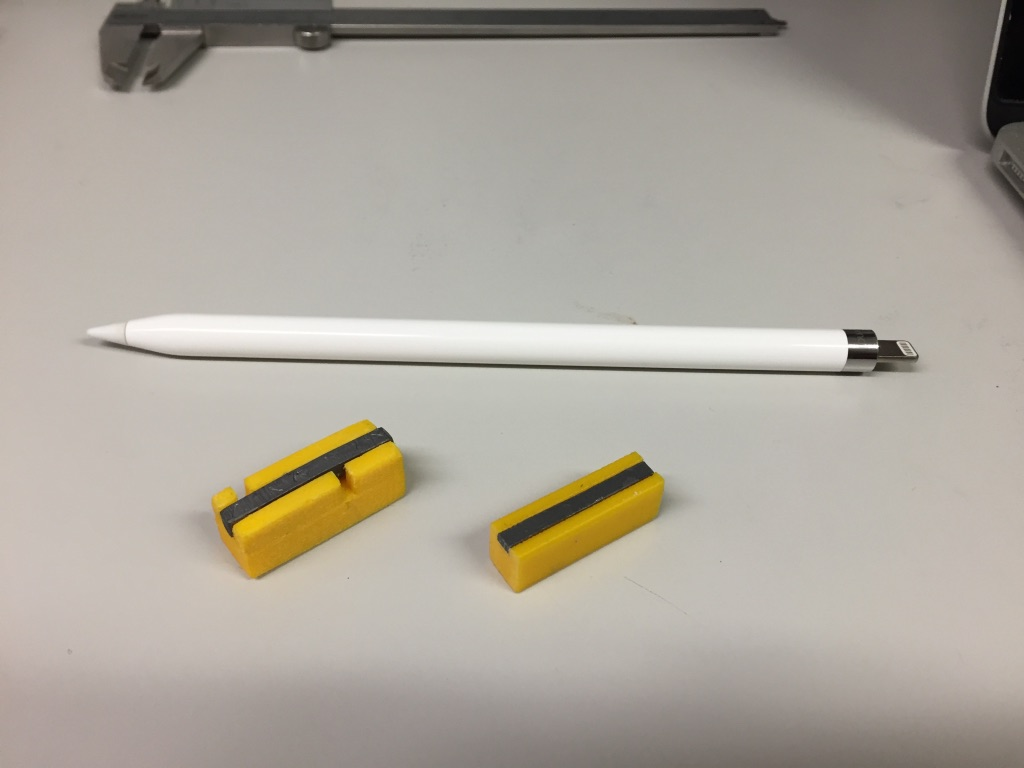
\includegraphics[width=4cm]{plots/lead1}
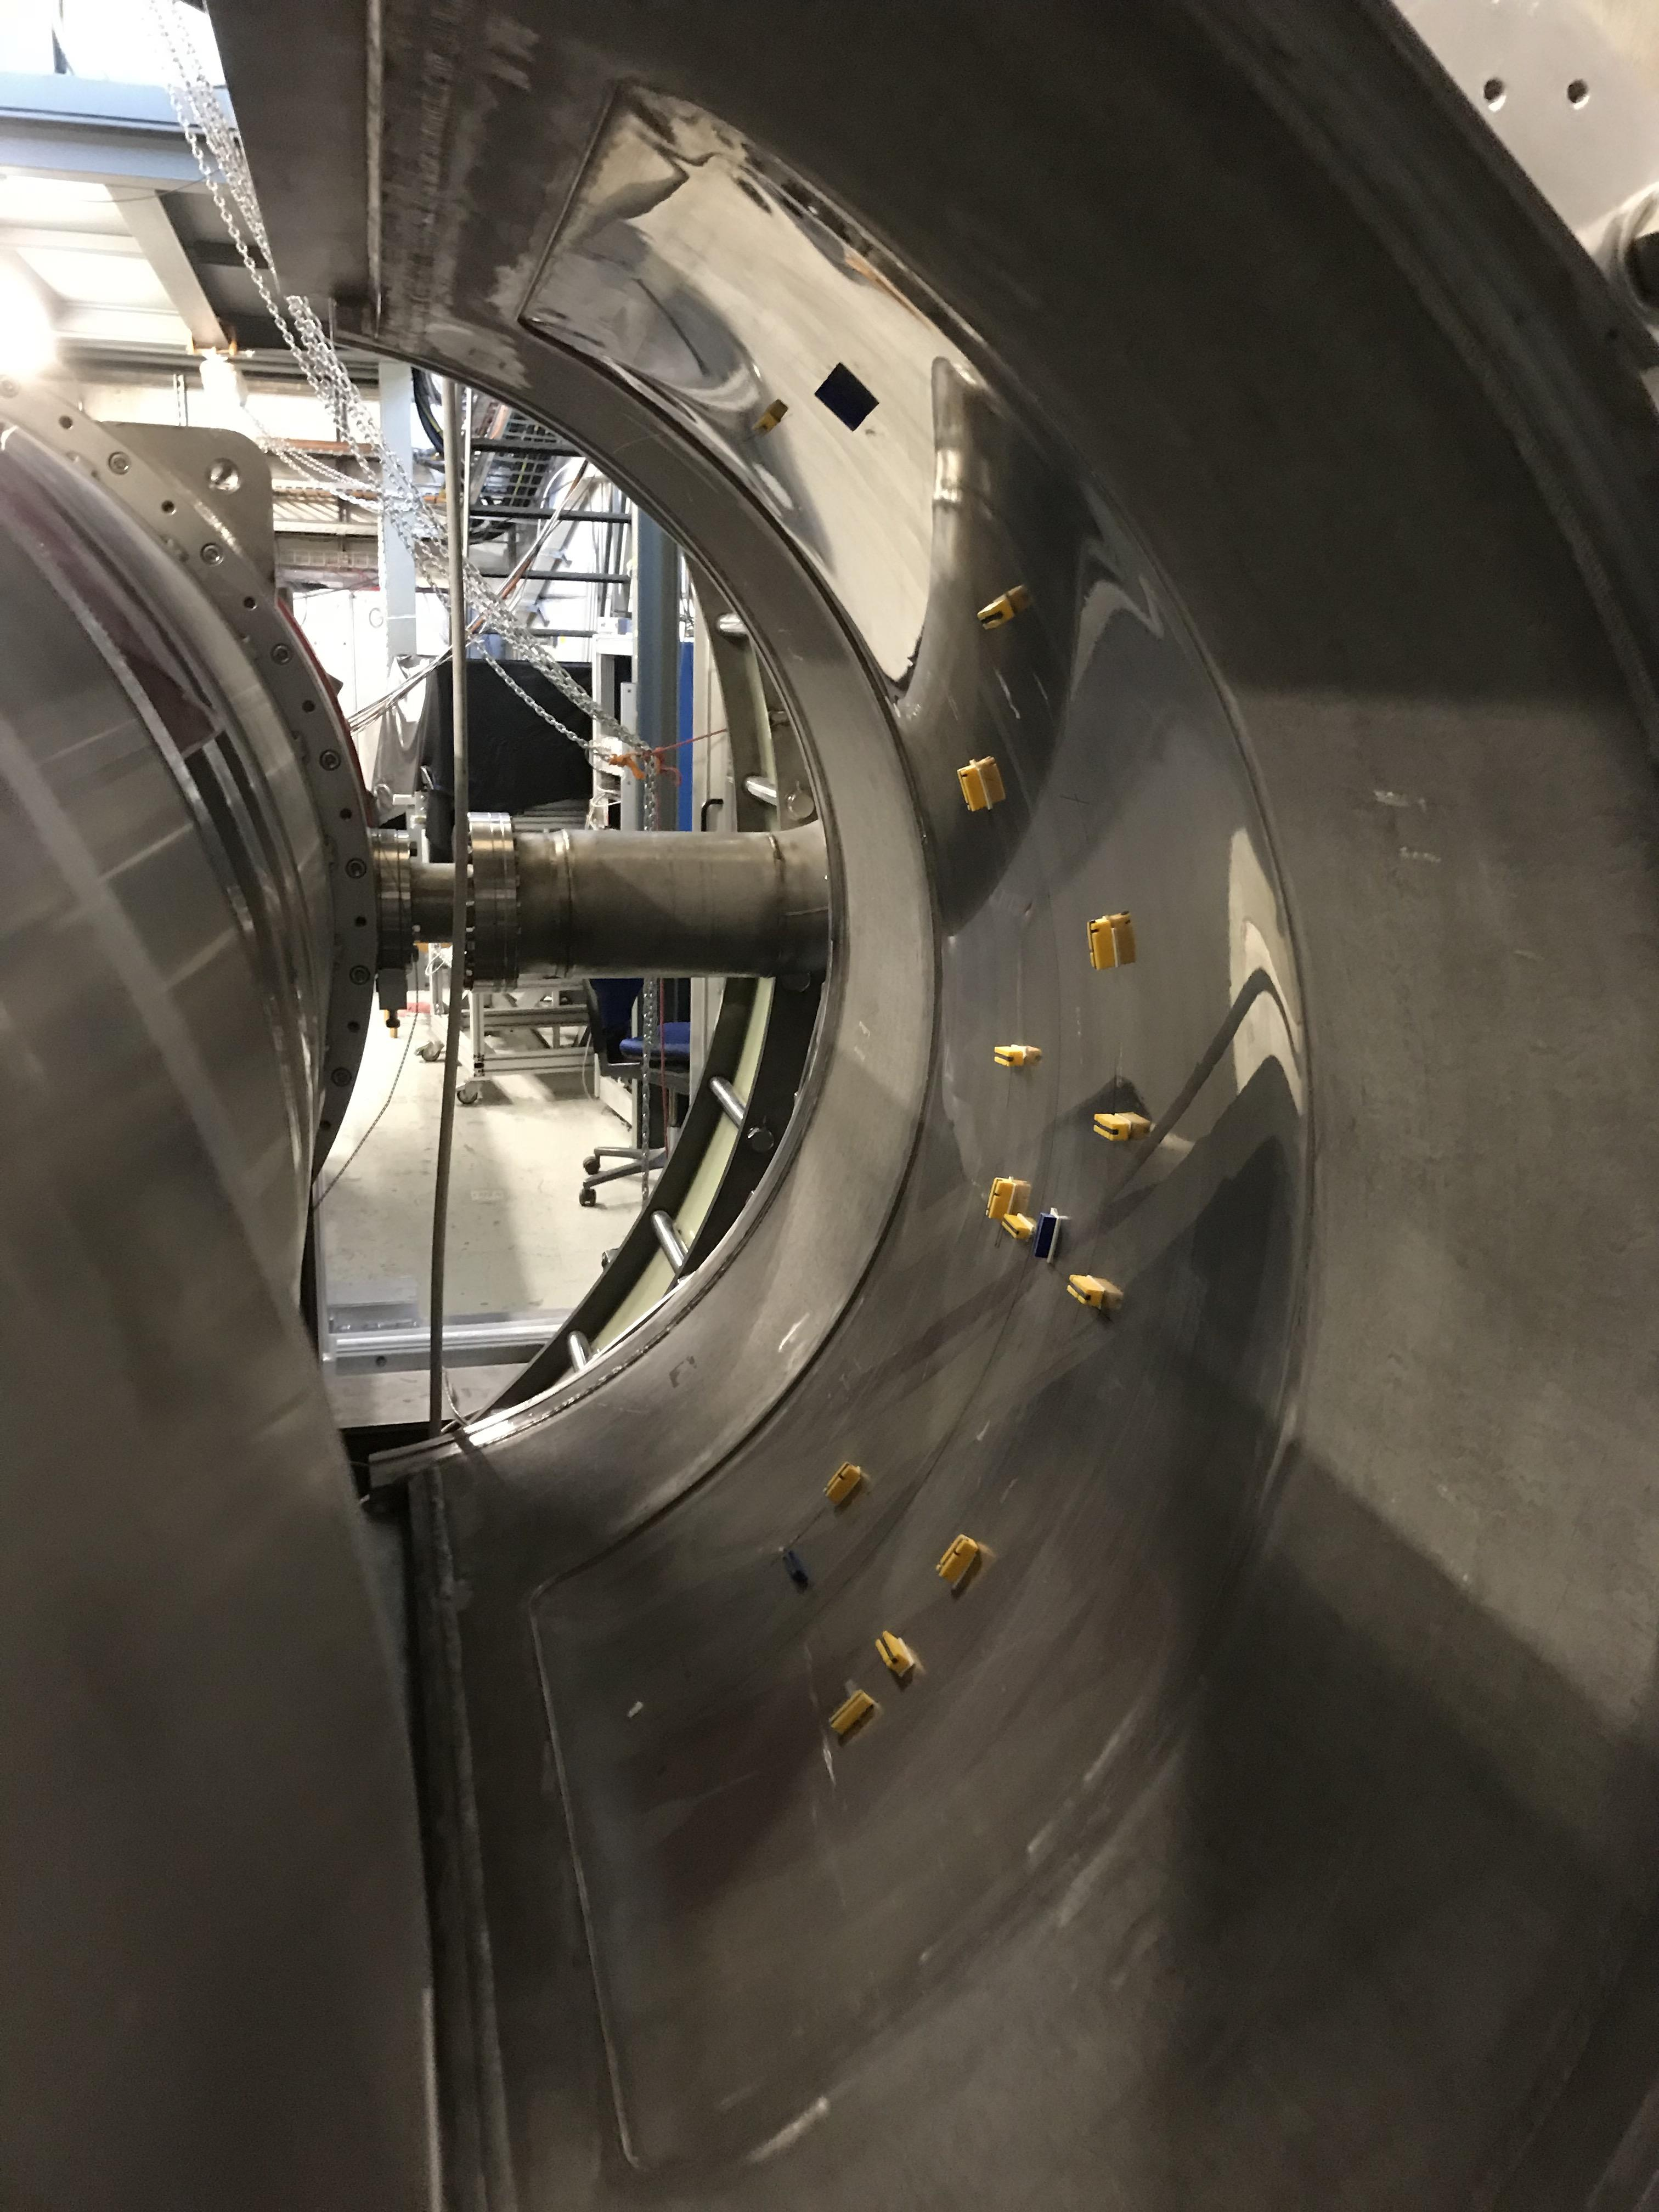
\includegraphics[width=4cm]{plots/MountedLeadStrips3}
\caption{Lead absorber strips mounted on the inner face
of LXe cryostat. [change lead strip photo]}
\label{fig:lead1} 
\end{figure}
\begin{figure}[]
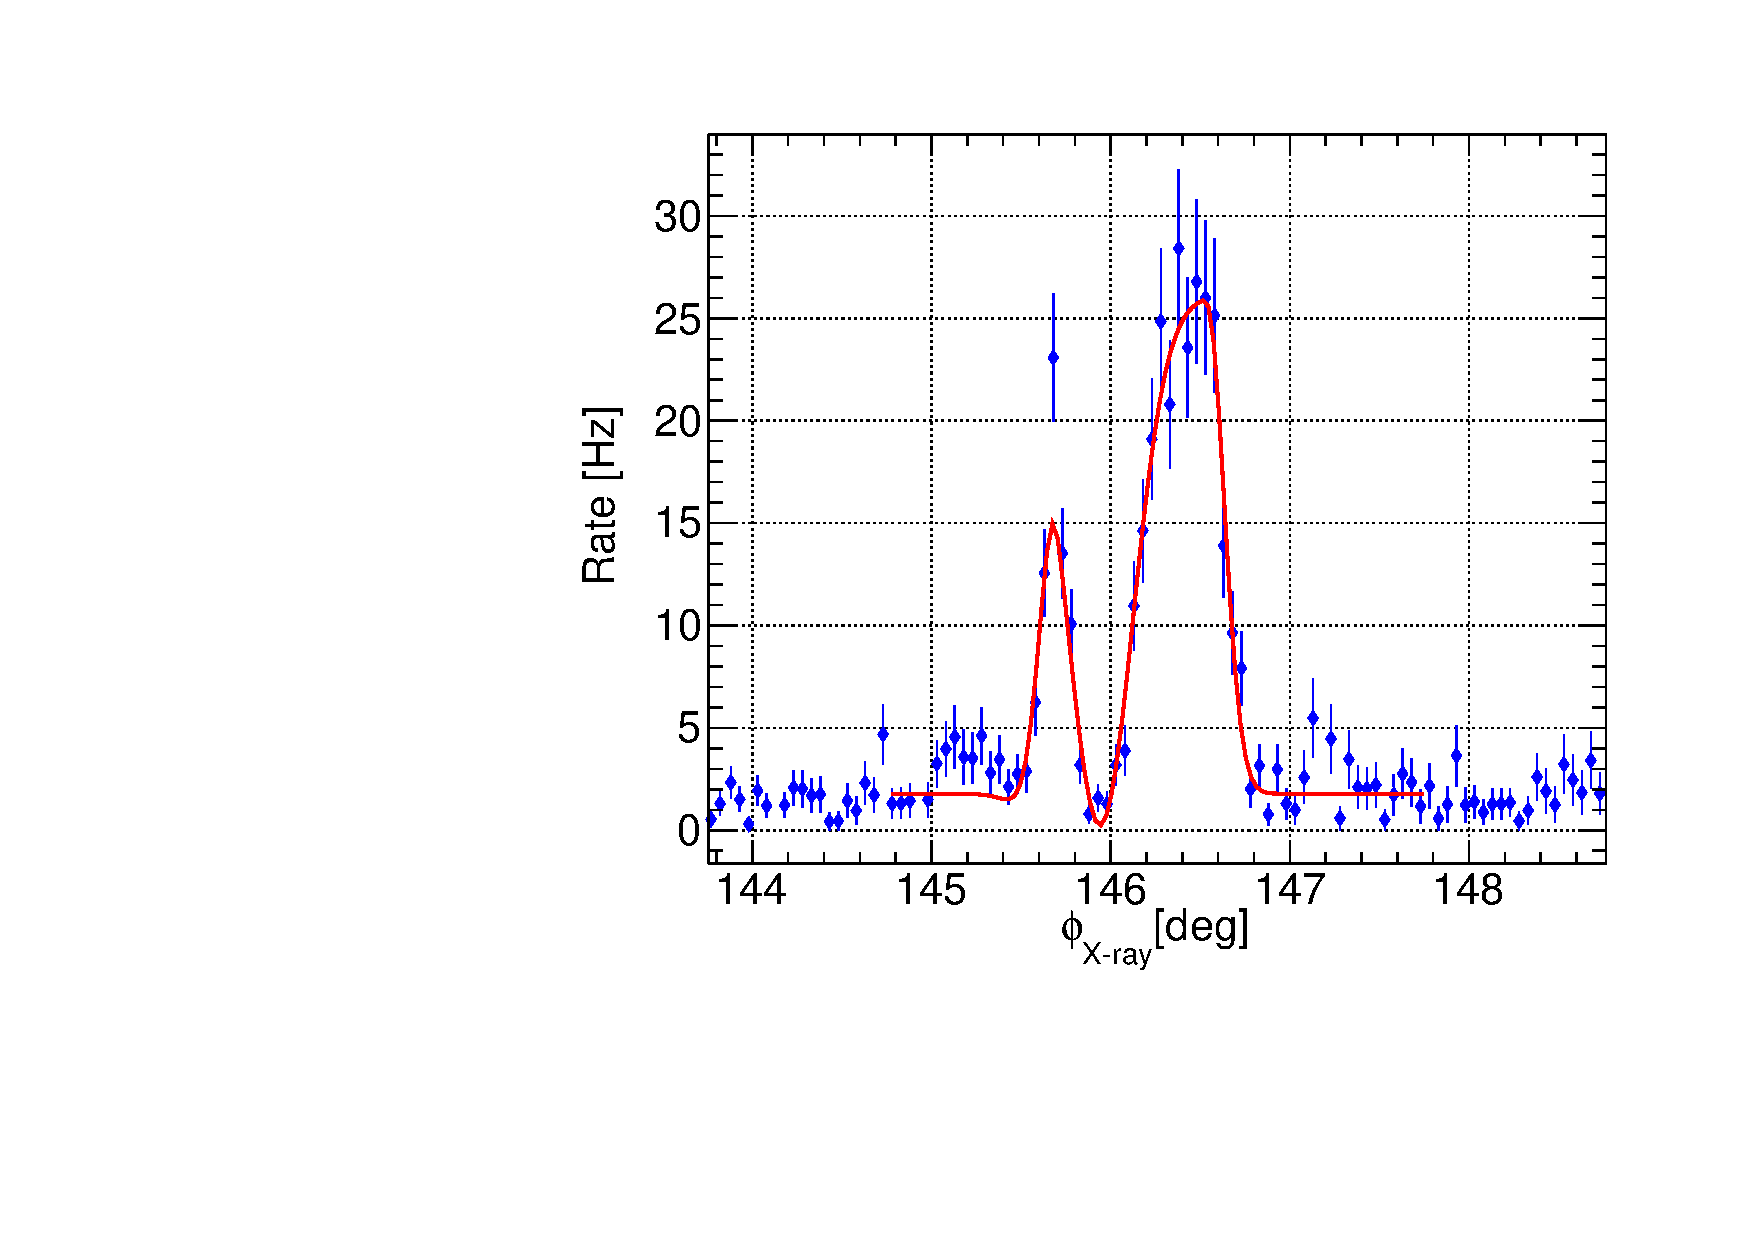
\includegraphics[width=4cm]{plots/2018/MPPCLeadScan}
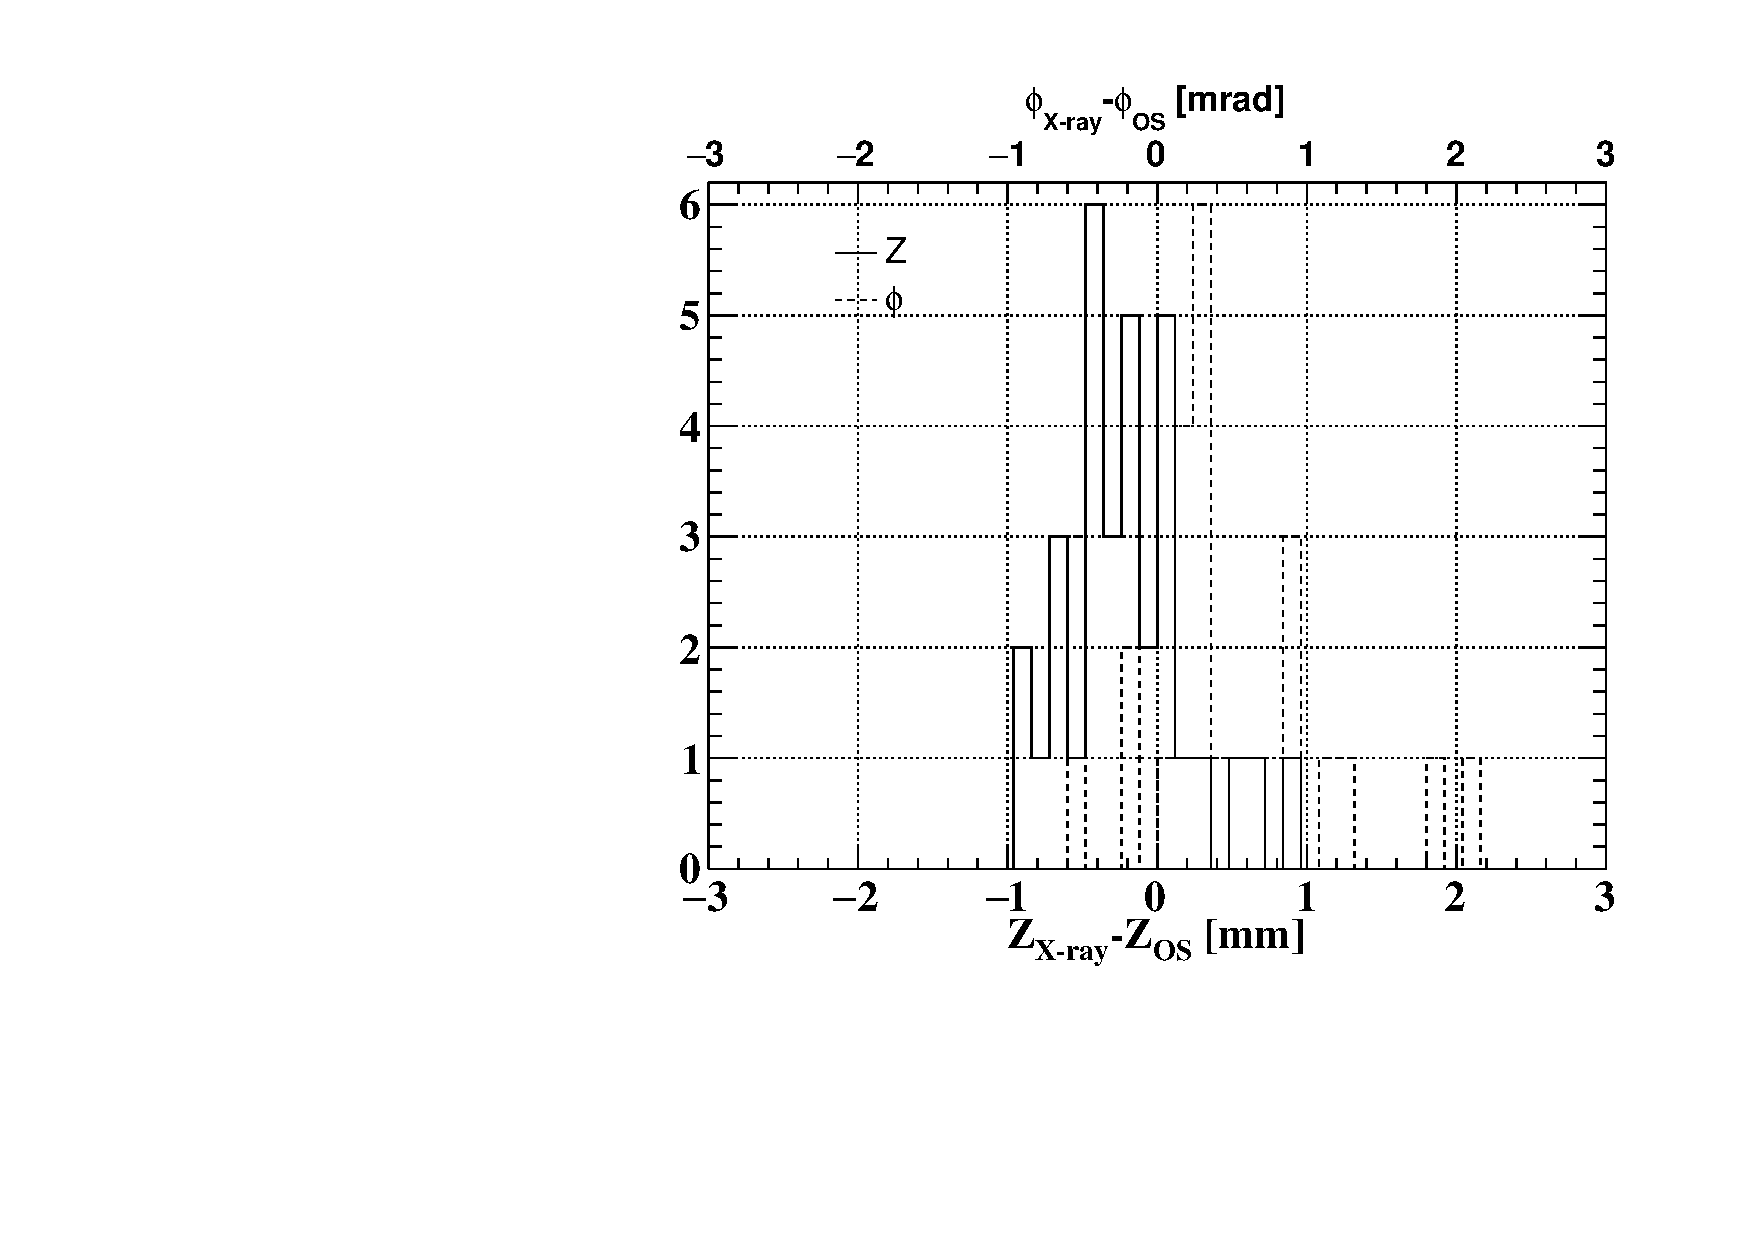
\includegraphics[width=4cm]{plots/2018/dzdphi_lead}
\caption{X-ray event rate recorded by a photodetector 
with reduction of events (shadow) due to the lead absorber strip
(left). The  comparison between strip positions calculated
with X-ray and optical surveys (right). }
\label{fig:lead2} 
\end{figure}


\subsection{Results}

